% IEEEtran selects the Type 1 ptm, phv, and pcr families while it loads.
% XeTeX and LuaTeX (tectonic is XeTeX-based) have no TU-encoded shapes for
% them, so those names are substituted silently here. The OpenType fonts are
% set after the class loads. pdfLaTeX skips this block.
\RequirePackage{iftex}
\iftutex
  \DeclareFontFamilySubstitution{TU}{ptm}{lmr}
  \DeclareFontFamilySubstitution{TU}{phv}{lmss}
  \DeclareFontFamilySubstitution{TU}{pcr}{lmtt}
\fi
\documentclass[conference]{IEEEtran}
\IEEEoverridecommandlockouts

% --- Packages -------------------------------------------------------------
\usepackage{cite}
\usepackage{amsmath}
% Times text and math. pdfLaTeX uses mathptmx. XeTeX and LuaTeX load the
% OpenType TeX Gyre clones of Times, Helvetica, and Courier by file name, and
% TeX Gyre Termes Math.
\iftutex
  \usepackage{unicode-math}
  \setmainfont{texgyretermes}[Extension=.otf, UprightFont=*-regular,
    BoldFont=*-bold, ItalicFont=*-italic, BoldItalicFont=*-bolditalic]
  \setsansfont{texgyreheros}[Extension=.otf, UprightFont=*-regular,
    BoldFont=*-bold, ItalicFont=*-italic, BoldItalicFont=*-bolditalic]
  \setmonofont{texgyrecursor}[Extension=.otf, UprightFont=*-regular,
    BoldFont=*-bold, ItalicFont=*-italic, BoldItalicFont=*-bolditalic]
  \setmathfont{texgyretermes-math.otf}
\else
  \usepackage{mathptmx} % Times text and math available in the build environment
\fi
\usepackage{array}
\usepackage{booktabs}
\usepackage{url}
\usepackage{xcolor}
\usepackage{tikz}
\usetikzlibrary{arrows.meta,positioning,calc}
\usepackage{pgfplots}
\pgfplotsset{compat=1.18}
\usepackage[hidelinks]{hyperref}

% Standard TeX hyphenation. Compound modifiers are hyphenated in the source
% (capability-first, redact-then-sign); em dashes are still avoided in prose.
% Long unbreakable \code{} identifiers still need extra stretch on some lines.
\tolerance=3000
\emergencystretch=3em

% IEEEtran prints "Abstract" and "Index Terms" followed by an em dash. Replace that
% separator with a colon so no dash appears in the running text.
\usepackage{etoolbox}
\patchcmd{\abstract}{\textit{\abstractname}---\relax}{\textit{\abstractname}:\ }{}{}
\patchcmd{\IEEEkeywords}{\textit{\IEEEkeywordsname}---\relax}{\textit{\IEEEkeywordsname}:\ }{}{}

% TikZ styles shared by the figures.
\tikzset{
  lbox/.style={draw, rounded corners=2pt, align=center, font=\scriptsize,
               text width=17mm, minimum height=9mm, inner sep=2pt, fill=blue!5},
  iobox/.style={lbox, fill=black!8},
  cbox/.style={lbox, fill=green!8},
  stepbox/.style={draw, rounded corners=2pt, align=center, font=\scriptsize,
               text width=58mm, minimum height=6mm, inner sep=3pt, fill=blue!5},
  flow/.style={-{Latex[length=2mm]}, semithick},
}

\newcommand{\code}[1]{\texttt{\small #1}}

\begin{document}

\title{Lattice: Signed, Replayable Capability Receipts for Model Runs}

\author{\IEEEauthorblockN{Lakshman Turlapati\IEEEauthorrefmark{1}}
\IEEEauthorblockA{Full Self Browsing\\
\url{https://github.com/fullselfbrowsing/Lattice}\\
Alumnus, Naveen Jindal School of Management,\\
The University of Texas at Dallas (M.S., December 2025)}
\and
\IEEEauthorblockN{Rabih Neouchi}
\IEEEauthorblockA{Naveen Jindal School of Management\\
The University of Texas at Dallas, Richardson, Texas, USA\\
Rabih.Neouchi@UTDallas.edu}
\thanks{\IEEEauthorrefmark{1}Corresponding author.
% TODO(corresponding-author): personal email. The UTD netid is not used.
}}

\maketitle

% --- Abstract -------------------------------------------------------------
\begin{abstract}
Production systems built on large language models usually keep a free-text log of a run.
Lattice is a capability-first TypeScript runtime. When a signer is configured,
\code{ai.run} and multi-agent crews emit capability receipts. A receipt commits to hashes
of the input artifacts and the output, a hash of the contract, and the selected route. It
does not commit to the task text, the policy, or the reasons a route was chosen. The body
is canonicalized with RFC 8785, matched personal data is masked before signing, and the
envelope is signed with Ed25519. Routing is a deterministic function, and a violated
output invariant is terminal. An offline evaluation against mocked providers measures
signing cost, receipt size, tamper rejection, and whether a kept output still matches its
signed hash. Audience and nonce binding, a schema-version floor, and a chain-length check
are verifier opt-ins. A crew's closing receipt lists every other member of its chain, so a
verifier that enforces closure rejects a dropped leaf.
\end{abstract}

\begin{IEEEkeywords}
capability receipts, verifiable replay, LLM orchestration, software supply chain,
canonical JSON, digital signatures, reproducibility, audit trails
\end{IEEEkeywords}

% --- Introduction ---------------------------------------------------------
\section{Introduction}

Software that calls large language models has moved from prototypes into systems
that approve refunds, triage insurance claims, route field operations, and process
medical and recruiting documents. These systems combine text with images, audio,
documents, structured outputs, and tool calls, and they increasingly spread a
single task across several model providers for cost, latency, privacy, or
capability reasons. As the stakes rise, two questions follow every run. First, can
an operator or an auditor trust the record of what happened. Second, can anyone
later check, offline and without trusting whoever stored the record, that a kept
input or output is the one the run used or returned. Today the honest answer to both
questions is usually no.

The reason is structural. The dominant integration libraries are provider wrappers.
They normalize the shape of a chat or generation call across vendors and they
provide convenience around tools, memory, and agents. They do not produce a
tamper-evident record of a run, they do not return a deterministic and
inspectable account of why one model was chosen over another, and they do not let a
third party check a kept result against a signed artifact. A free
text log is not a proof. It can be edited after the fact, it does not bind the
inputs to the outputs, and it carries no signature that a verifier can check with a
public key.

This paper argues that the missing primitive is a per-run, signed, replayable
\emph{capability receipt}, and that a runtime can make such a receipt a default
byproduct of normal operation rather than an after-the-fact instrumentation task.
We build this argument concretely through Lattice, a capability-first runtime SDK
written in TypeScript. A developer describes the job, supplies any mix of artifacts,
declares the desired outputs and policy constraints, and optionally attaches a
contract. Lattice then routes the work deterministically, packs context, prepares
artifacts for the chosen provider, and enforces output invariants. When a signer is
configured, \code{ai.run} emits a receipt on every outcome, success or failure, and a
multi-agent crew emits a chain of receipts. The single-agent loop, \code{ai.runAgent},
returns no receipt.

Lattice provides four guarantees that together make a run auditable and
reproducible.

\begin{enumerate}
\item \textbf{Deterministic and inspectable routing.} The router is a pure function
of the capability catalog, the request, and the policy. It uses hard filters, a
stable score, and a deterministic tie break, and its execution plan reports the full
set of candidates, the rejected candidates, the fallback chain, and a typed list of
reasons when no route is possible. There is no randomness and no model call inside
routing. The receipt signs only the selected route.
\item \textbf{Terminal output invariants.} Output level tripwires such as
``must cite an artifact'' or ``no matched email, social security, phone, or card
number'' are evaluated by a pure kernel. A violation produces a terminal error that the fallback chain is
forbidden to retry, which prevents a system from quietly trying again until a banned
output slips through.
\item \textbf{Signed capability receipts.} With a signer, every \code{ai.run}
outcome and every crew run emits receipts that are canonicalized with RFC 8785,
redacted before signing, and signed with Ed25519 inside a Dead Simple Signing
Envelope. A receipt binds hashes of the input artifacts and the output, the contract
hash, and the selected route to a key, through a signature that any holder of the
public key can check.
\item \textbf{Offline replay as output binding.} A receipt and its
content-addressed artifacts can be materialized into a replay envelope.
Materialization verifies the signature before it loads any artifact. Replay does not
call a model: it recomputes the hash of the recorded output and compares it with the
value the receipt commits to, and a property test checks that round trip.
\end{enumerate}

We make the following contributions. We define the capability receipt as a signing
and replay primitive for model runs, and we show how a redact-then-sign
ordering and a canonical encoding turn it into a verifiable artifact rather than a
log line. We show how a deterministic and inspectable router, terminal output
invariants, and a content-addressed verification tool compose into a runtime where
auditability and reproducibility are default properties. We describe a working
implementation that ships publicly with supply-chain provenance, modular adoption
paths, a seven-provider parity contract, and a test suite that encodes the
guarantees as invariants. We also show how external executors can mint compatible
receipts without adopting Lattice's provider or agent runtime. The remainder of the
paper covers background and related work, the threat model and goals, the design, the
implementation, the evaluation, a discussion, the limitations, future work, and a
conclusion.

% --- Background and Related Work ------------------------------------------
\section{Background and Related Work}

\subsection{Provider wrappers and agent frameworks}

A first family of systems normalizes model access. The Vercel AI SDK
\cite{vercelaisdk} offers a broad provider-agnostic TypeScript toolkit with
multimodal generation, tools, and agents. LangChain and LangGraph \cite{langchain}
provide orchestration, sessions, and tracing. LiteLLM \cite{litellm} is strong
routing infrastructure that exposes a common interface across many providers with
fallback and gateway features. The OpenAI Agents SDK \cite{openaiagents} provides
agent loops, sessions, and tool-use. The Model Context Protocol \cite{mcp}
standardizes how tools and context attach to a model session. These systems are
valuable and widely used. None of them, however, emit a signed and replayable per
run receipt. Their tracing is observability for humans, not a cryptographic artifact
that a third party can verify against a public key, and their routing is generally
either configuration driven or model chosen rather than a deterministic pure
function whose full decision is returned for inspection.

\subsection{Software supply-chain provenance}

A second family secures the provenance of software artifacts. in-toto
\cite{intoto} provides end-to-end guarantees over a software supply chain by signing
the steps that produced an artifact. The Dead Simple Signing Envelope \cite{dsse}
defines a minimal envelope and a pre-authentication encoding so that signatures
commit unambiguously to a payload and its type. Sigstore \cite{sigstore} makes
signing and transparency broadly accessible. SLSA \cite{slsa} defines levels of
supply chain integrity, and The Update Framework \cite{tuf} addresses survivable key
compromise in update systems. Lattice borrows directly from this lineage. It reuses
the DSSE envelope and pre-authentication encoding, it adopts a key set with explicit
key states in the spirit of key rotation and revocation, and it treats the published
package itself as a supply chain artifact with provenance attestations. The novelty
is to apply this provenance discipline not to a build, but to an individual model run
at runtime.

\subsection{Canonicalization and signatures}

Signing a structured object requires a deterministic byte encoding, otherwise two
semantically equal objects can produce different signatures. The JSON Canonicalization
Scheme \cite{rfc8785} defines such an encoding for JSON, and the I-JSON message format
\cite{rfc7493} constrains JSON to an interoperable subset, which matters for how
numbers and floats are serialized. Lattice canonicalizes receipts with RFC 8785 and
serializes monetary cost as an I-JSON string so that receipts never carry raw floats.
Signatures use EdDSA \cite{rfc8032}, the elliptic curve signature construction that is
widely deployed for compact and fast signatures.

\subsection{Transparency and reproducibility in machine learning}

A third family documents models and data for accountability. Model Cards
\cite{modelcards} and Datasheets for Datasets \cite{datasheets} standardize
disclosure about a model or dataset, and reproducibility programs in the research
community \cite{reproml} push toward runs that others can repeat. These efforts
describe an artifact or a study. A capability receipt is complementary and finer
grained. It describes a single production run and makes that run independently
checkable and replayable. Merkle trees \cite{merkle} provide a standard way to commit
to a set of items with a single root; a Lattice receipt uses one for its signed lineage
root over the artifacts that a run consumed and produced.

\subsection{Signed receipts for agent actions}

Four systems from 2026 target evidence for autonomous agent runs and are the closest
prior work. Sello \cite{figuera2026notarized} has the service that receives an agent's
call sign a receipt with its own Ed25519 key inside a COSE envelope, encrypt it to the
agent's owner, and publish it to a witnessed Merkle log; verification needs the log
inclusion proof and a key registry, inputs and outputs appear only as hashes, and the
protocol is independent of models and providers. Agent Flight Recorder
\cite{bindschaedler2026afr} is middleware that hash-chains agent events into Merkle
epochs and anchors epoch roots on a public chain; there is no per-event signature, a
verifier needs read access to the chain, and policy verdicts are recorded rather than
enforced. NovaFabric \cite{ardebili2026novafabric} captures traffic to several
providers into an operator-signed evidence bundle, with Ed25519 at the collector and an
ECDSA P-256 seal per tenant inside a DSSE envelope, that is designed for offline
verification with stock tools and supports four replay modes; its policy gates act on
promotion, export, and replay rather than on live runs, and its author describes the
implementation as experimental. Janus \cite{arslan2026janus} is the closest in spirit:
a single-node daemon appends each agent step's proposal, gate verdict, and validator
response to a hash-chained log whose segments it signs with Ed25519 before the step
runs or its effect is released, an auditor re-derives every verdict offline from the
log and one public key, and replay re-derived all 287 terminal sagas in the paper's
experiment; it does not choose models or providers, model decision records are
self-reported rather than signed, and effects on its SDK path are admitted
cooperatively rather than held. TrustTrack \cite{li2025trusttrack} is a vision paper
that proposes verifiable identity, policy commitments, and tamper-resistant behavioral
logs for multi-agent systems, without an implementation. Certificate Transparency
\cite{rfc6962,rfc9162} is the reference design for the log-based approach that Sello
and Agent Flight Recorder build on: it makes issuance auditable after the fact through
an append-only log, whereas a Lattice receipt is checkable on its own with a public key
and binds the selected route, the contract hash, and the output hash.
Table~\ref{tab:receipts} compares the four implemented systems with Lattice, and
Section~\ref{sec:realworld} runs each of them on the same recorded requests.

\begin{table*}[t]
\caption{Agent receipt systems compared with Lattice. The signer, policy, routing, and
multi-provider cells summarize each paper's own description; ``not stated'' means the
source does not say. The offline-verify and signed-output-binding cells agree with the
runs in Table~\ref{tab:rw-matrix}, which used a mock transparency log for Sello and a mock
chain anchor for Agent Flight Recorder. Signed output binding means the record is signed
and the system's own verifier rejects a byte edit.}
\label{tab:receipts}
\centering
\footnotesize
\setlength{\tabcolsep}{4pt}
\begin{tabular}{@{}>{\raggedright\arraybackslash}p{19mm}>{\raggedright\arraybackslash}p{28mm}>{\raggedright\arraybackslash}p{32mm}>{\raggedright\arraybackslash}p{24mm}>{\raggedright\arraybackslash}p{28mm}>{\raggedright\arraybackslash}p{15mm}>{\raggedright\arraybackslash}p{16mm}@{}}
\toprule
System & Signer & Offline verify & Signed output binding & Policy checks & Routing & Multi-provider \\
\midrule
Sello \cite{figuera2026notarized} & receiving service, Ed25519 in COSE & yes with a mock log; the paper's verifier needs a log inclusion proof and a key registry & yes; hashes only & no; service denials are recorded & no & not model specific \\
Agent Flight Recorder \cite{bindschaedler2026afr} & none per event; ECDSA on the chain anchor & yes with a mock anchor; the paper's verifier reads the chain & no; events are hash-chained, not signed & no; verdicts logged & no & not stated \\
NovaFabric \cite{ardebili2026novafabric} & operator; collector Ed25519 and tenant ECDSA seal & yes for a sealed capsule with a self-asserted key & yes for the sealed capsule; no for the HMAC record & partial; gates on export and replay & no & yes, capture \\
Janus \cite{arslan2026janus} & log daemon and participants, Ed25519 & yes; log and one public key & yes; signed log segments & yes; pre-execution and pre-release gates & no & not stated \\
Lattice & runtime signer over a key set, Ed25519 in DSSE & yes; public key only & yes; signed output hash & yes; invariants, budgets, and policy at run time & yes; deterministic, selected route signed & yes; seven adapters \\
\bottomrule
\end{tabular}
\end{table*}

\subsection{The gap}

Across these families, and to our knowledge, Lattice is the first open SDK that
combines per-run signed receipts, deterministic routing, run-time policy enforcement,
and signed output binding in one runtime. The provider wrappers and agent frameworks
route and orchestrate but do not sign; the supply chain systems sign and verify offline
but know nothing about model runs; and the agent receipt systems in
Table~\ref{tab:receipts} sign and verify evidence, with Janus also gating effects
and replaying decisions, but none of them chooses the model, so their evidence is never
bound to a selected route. The receipt design first appears in the repository's
public history in commit \code{fa6d5a1} of May 11, 2026 \cite{lattice}, before the Sello (June 2026)
and the Agent Flight Recorder, NovaFabric, and Janus (September 2026) preprints. The
audience, nonce, and expiry fields, chain verification, and chain closure were added in
October 2026, after those preprints.

% --- Threat Model and Goals -----------------------------------------------
\section{Threat Model and Goals}

\subsection{Actors and trust assumptions}

We consider four actors. The \emph{issuer} is the Lattice runtime that performs a
run and signs a receipt with a private key. The \emph{provider} is an external model
service that the runtime calls and that we treat as untrusted and possibly buggy. The
\emph{verifier} is any party that later receives a receipt and wishes to check it,
possibly without trusting the issuer at the time of verification. The
\emph{adversary} may sit between these actors or may hold material that looks
legitimate.

\subsection{Adversary capabilities}

We assume an adversary who can tamper with a stored receipt, a transcript, or a
claimed output after a run completes. We assume an adversary who can attempt to
substitute a different model route while presenting a receipt that attests to the
intended route. We consider an adversary who has obtained a valid signing key and who
then tries to mint a receipt in an older schema in order to bypass integrity fields
that newer schemas commit to, a schema downgrade attack. We consider an adversary who
replays a valid receipt from a different run, a different relying party, or an
earlier time and presents it as proof of the current run. We also consider a careless
issuer whose run inputs contain secrets or personally identifiable information that
must never be embedded in a signed and shareable artifact.

\subsection{Security goals}

The runtime targets five goals. First, integrity of the run record: a receipt that
has been altered must fail verification. Second, non-repudiation through signature:
a verifier with the public key can confirm which key signed a receipt and whether
that key is active, retired, or revoked. Third, redaction before signing: personal
data matched by a detector, and the tripwire message that would otherwise quote it, are
reduced to a detector name, a length, and a mask before the canonical bytes are
produced. The signing key and the provider credential are not receipt fields. A
free-text field the caller chooses to store is the caller's responsibility. Input and
output hashes are unsalted SHA-256, so they hide high-entropy values only: anyone who
holds a receipt can confirm a guessed low-entropy value, such as a social security
number or a yes or no decision, by hashing candidates. Fourth, determinism for replay: a
verifier can recompute the hash of the recorded output and compare it to the value the
receipt commits to. Fifth,
downgrade resistance: a receipt in the original schema, or below a caller-supplied
\code{minVersion} floor, is rejected before any cryptographic work. Without that
floor, a v1.1 receipt still verifies.

\subsection{Non goals}

Several properties are explicitly out of scope. We do not provide confidentiality of
provider traffic, which is the responsibility of transport security. We do not
reproduce the live behavior of a remote model, since model providers are
nondeterministic and outside our trust boundary. Replay checks the recorded output
against its signed hash; it is not a fresh call to the provider. A signature alone proves
integrity and attribution, not freshness: binding a receipt to a relying party, a
nonce, or a validity window requires the optional v1.4 fields and the matching
verifier options described under verification below, and a verifier that must
accept a receipt only once keeps its own record of accepted content identifiers.
Dropping leaf receipts from an open receipt tree leaves a smaller tree that still
verifies. The chain verifier then returns a \code{tail-truncation-unchecked} warning
unless the caller passes an expected count. A crew run closes its tree instead: its root
declares closure and its last receipt lists the content identifiers of every other
member, so a dropped leaf or a dropped closer fails verification without an out-of-band
count under a verifier that enforces closure (Section~\ref{sec:chains}). We also
do not operate a hosted control plane. Lattice is a runtime SDK, and the receipt is a
portable artifact that travels with the run rather than a record locked inside a
service.

% --- Design ---------------------------------------------------------------
\section{Design}

Figure~\ref{fig:arch} shows the end-to-end run lifecycle that produces and then
consumes a capability receipt. The subsections that follow walk through each stage.

\begin{figure*}[t]
\centering
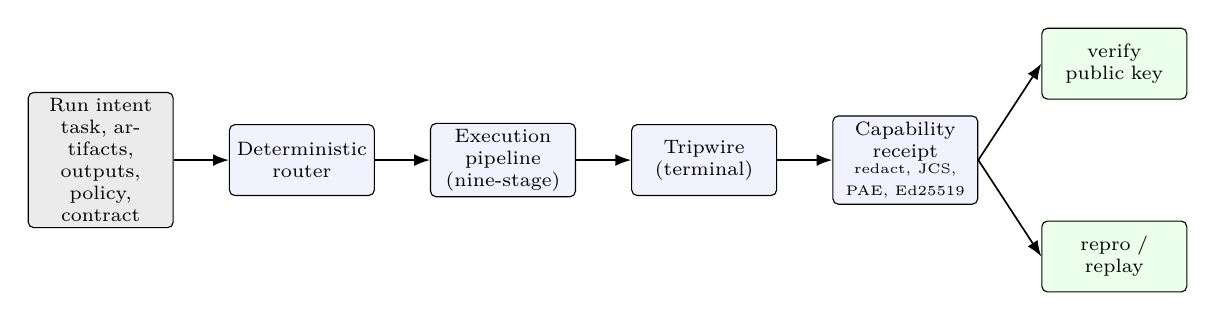
\begin{tikzpicture}[node distance=6mm and 7mm]
  \node[iobox] (intent) {Run intent\\ task, artifacts,\\ outputs, policy,\\ contract};
  \node[lbox, right=of intent] (router) {Deterministic\\ router};
  \node[lbox, right=of router] (exec) {Execution\\ pipeline\\ (nine-stage)};
  \node[lbox, right=of exec] (trip) {Tripwire\\ (terminal)};
  \node[lbox, right=of trip] (rcpt) {Capability\\ receipt\\ \tiny redact, JCS,\\ \tiny PAE, Ed25519};
  \node[cbox, above right=2mm and 8mm of rcpt] (verify) {verify\\ public key};
  \node[cbox, below right=2mm and 8mm of rcpt] (repro) {repro /\\ replay};
  \draw[flow] (intent) -- (router);
  \draw[flow] (router) -- (exec);
  \draw[flow] (exec) -- (trip);
  \draw[flow] (trip) -- (rcpt);
  \draw[flow] (rcpt.east) -- (verify.west);
  \draw[flow] (rcpt.east) -- (repro.west);
\end{tikzpicture}
\caption{The Lattice run lifecycle. A run intent is routed by a deterministic and
inspectable function, executed through a nine-stage pipeline, checked by terminal
output invariants, and committed to a signed capability receipt. The receipt is later
consumed by offline verification and by the \code{repro} check of a kept output
against the signed output hash.}
\label{fig:arch}
\end{figure*}

\subsection{The capability-first run model}

A run is described by a small intent: a \code{task} string, a set of \code{artifacts}
that may be text, JSON, images, audio, documents, or tool results, a map of declared
\code{outputs} with their schemas, a \code{policy} that expresses privacy, latency,
provider allow and deny lists, and budget, and an optional \code{contract}. The
developer does not select a model. The runtime selects one from a capability catalog
and records the decision in the execution plan. The receipt signs the selected route
next to hashes of the input artifacts, the output, and the contract. The task text and
the policy are not signed, so a receipt shows which route served a run and which inputs
and outputs it bound, not what the run was asked to do. How an artifact reaches the
model depends on the provider adapter (Section~\ref{sec:parity}).

\subsection{Deterministic and inspectable routing}

Routing is implemented as a pure function, \code{routeDeterministically}, that takes
the capability catalog, the request, and the policy and returns a route decision. It
performs no input or output, draws no randomness, and never calls a model. The
function first applies hard filters that reject a candidate when the provider is
unavailable, when an explicit provider or model override does not match, when a
required input or output modality is unsupported, when structured output is required
but unsupported, or when the estimated input exceeds the context window. It then
applies policy filters that reject on an allow or deny list, on a privacy class, on a
no-logging or no-upload requirement, on a latency class, or on a budget ceiling.
Surviving candidates are scored from cost, latency, and context headroom, and ties
are broken by a stable order over acceptance status, score, provider name, and model
name, with names compared by code unit rather than by locale so the order is the same
on every machine. The catalog position is deliberately not part of the score, so the
decision does not depend on the order in which providers were registered; a test evaluates
every permutation of a near-equal-cost catalog and requires the same selected route
and the same fallback chain. The decision exposes the selected route, all candidates, all
rejected candidates, a fallback chain of policy-preserving alternatives, and a
deduplicated list of typed reasons when no route is possible. The full execution plan
is stable JSON with a nine-stage pipeline: analysis, transforms, context packing,
provider packaging, tool execution, execution, validation, tripwire, and persistence.
The execution plan returns this decision in full. The receipt signs only the
selected route, as a provider identifier, a capability identifier, and an attempt
number, and not the candidates, the scores, or the policy, so it attests to which
route served the run but not to why that route was chosen. Because the router is a pure
function, a reviewer who holds the same catalog, request, and policy can reproduce the
decision by re-running it.

\subsection{Output invariants with terminal semantics}

Lattice lets a developer attach output invariants through a fluent builder,
\code{inv}, with constructors \code{mustCite}, \code{fieldFromTable}, \code{noPII},
and \code{matches}, where the last validates against a Standard Schema
\cite{standardschema}. These invariants are evaluated by a pure kernel,
\code{evaluateTripwires}, that performs no input or output, reads no clock, and uses
no randomness, so the same output and the same invariants always yield the same
result. The kernel aborts on the first violation. It scans strings and walks nested
objects, arrays, and wildcard paths in a deterministic order, so a value buried inside
a structured output is not missed.

The default \code{noPII} detectors are regular expressions for four formats. An email
address matches as written, and so do a dashed United States social security number
(\code{ddd-dd-dddd}) and a separated ten-digit United States phone number. A spaced or
undashed nine-digit number counts as a social security number only when an SSN cue
such as \code{ssn} or \code{social security} is the nearest preceding word. A plain
ten-digit run counts as a phone number only when it is a valid North American number
that follows a phone cue such as \code{phone} or \code{call}, or a \code{+1} or
\code{1-} trunk prefix. A card number is 13 to 19 digits, optionally grouped by
single spaces or dashes, that pass the Luhn checksum; runs that start with 0 or 1, and 13-digit runs
that start with an ISBN-13 prefix, are skipped. A social security, phone, or card
candidate is also skipped when the nearest preceding word on the same line is an
identifier label: order, invoice, sku, ref, po, isbn, txn, or one of a few
abbreviations. A phone number with a trunk prefix is flagged even after a label, and
labels do not affect email addresses. Ordinary words such as customer,
account, ticket, or id are not labels. These rules trade recall against precision in
known ways. A real value right after a label (``ref 123-45-6789'') is missed, and so is
a bare nine- or ten-digit value without its cue. A value under a telling object key,
such as \code{\{ssn: "123456789"\}}, is missed because the detectors read string values,
not field names. In the other direction, about one random long digit run in ten passes
the Luhn check, so a text that lists $k$ long numeric identifiers is flagged with
probability near $1-0.9^k$. Names, street addresses, and non-United States formats are
not detected.

By default \code{mustCite(name)} is a structured check. The output's top-level
\code{citations} list, or else its \code{evidence} list, must contain the artifact name
as a string entry or as an object entry whose \code{source} key, or another configured
key, equals it. When neither top-level list names the artifact, nested
\code{citations} and \code{evidence} lists are searched as well, unless the invariant
declares a path to the list. The default never reads prose. Three options extend it.
With \code{inline}, a bracket or parenthesis group whose content, or one comma- or
semicolon-separated part of it, equals the name counts when no located list has
entries; code spans and link text are ignored. With \code{rejectUncited}, a list entry
that names the artifact is rejected when the prose carries square-bracket citations,
such as \code{[1]}, \code{[Smith 1999]}, or a list entry's identifier, and none of them
resolves to the artifact. \code{textPath} limits both scans to one field. Each option
enters the contract declaration only when set, so an existing contract keeps its hash.
The check stays syntactic. By default an answer passes when its list names the
artifact even if its text cites nothing. \code{inline} also accepts a marker in a
sentence that disowns the source. \code{rejectUncited} reads only square brackets, so a
parenthetical citation of another work goes unseen, and without \code{textPath} a
bracketed number in an unrelated string, such as a log line, counts as a citation. No
option judges whether the cited artifact supports the claim.

When a \code{noPII} invariant fires, the runtime error
returned to the caller carries the detector name and the matched substring so the
violation can be debugged, and the receipt redaction policy replaces that substring
with the detector name, the match length, and a shape mask before anything is signed;
the other three invariant kinds have their observed value reduced to a type label from a
closed set in the same step, and every kind's message is rebuilt from the invariant kind
and the declared path so that neither model produced object keys nor schema issue
text reach the signed bytes. A violation produces a \code{TripwireViolationError} that carries the
flag \code{terminal: true}. The predicate \code{isTerminal} returns true for a
tripwire violation and for a no contract match, and the fallback chain consults this
predicate so that a terminal failure is never retried. This matters for safety: a
system that retries until a banned output passes is worse than a system that fails
closed, and terminal semantics make failing closed the default.

\subsection{Capability contracts and preflight}

A contract expresses requirements that must hold before and around a run: a budget
with a maximum cost and, for agent runs, iteration and wall time caps, a set of
invariants, a quality floor, a set of required modalities, and a required privacy
class. A pure preflight evaluator, \code{evaluateContractAgainstRoute}, runs inside
the router and can reject a route with a typed reason such as a budget exceeded, a
missing modality, or a privacy mismatch. A quality floor reason is reserved for the
evaluation tool described later. Usage is normalized to prompt tokens, completion
tokens, and a cost in United States dollars on every outcome, success or failure, and
a null cost is distinct from a zero cost so that an unmeasured price is never confused
with a free call.

\subsection{The capability receipt}

The receipt is the central artifact. Its body records the requested and observed
model, the selected route, normalized usage, the contract verdict, the contract hash
(null without a contract), SHA-256 hashes of the input artifacts, the output hash, a
lineage root over the artifacts, and the redaction manifest, with optional audience,
nonce, expiry, parent, and chain-closure fields. The task text, the packed prompt, and
the policy are not part of it. Its construction enforces a strict ordering that is the
heart of the security argument. Figure~\ref{fig:pipeline} shows the pipeline, and
Figure~\ref{fig:envelope} shows the resulting envelope.

First, the runtime assembles the raw receipt body from the run record. Second, it
redacts the body. Redaction rewrites the tripwire evidence for every invariant kind,
replacing a matched personally identifiable value with a detector name, a length, and
a shape mask and reducing other observed values to a type label, and records a
manifest of redactions, each with a path and a reason, and a signed redaction policy
identifier whose default value is \code{lattice.default.v1}. Each manifest entry is
written at the moment of the corresponding rewrite, so the manifest cannot claim a
redaction that did not happen.
Third, it canonicalizes the redacted body with RFC 8785 \cite{rfc8785}. Fourth, it
base64 encodes the canonical bytes as the payload. Fifth, it builds the DSSE pre
authentication encoding over the payload type and the payload. Sixth, it signs the
pre-authentication encoding with Ed25519. The ordering is enforced structurally, not
by convention: the canonicalization function is only ever called on the output of the
redaction function, so a code path that signs unredacted bytes is unrepresentable.
This is what we mean by redact-then-sign as an architectural invariant rather than a
guideline.

\begin{figure}[t]
\centering
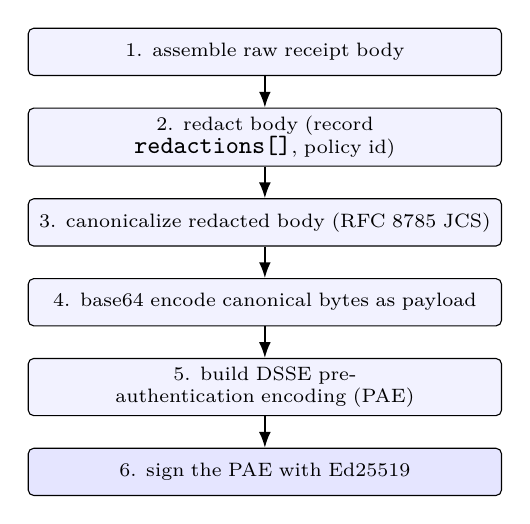
\begin{tikzpicture}[node distance=4mm]
  \node[stepbox] (s1) {1. assemble raw receipt body};
  \node[stepbox, below=of s1] (s2) {2. redact body (record \code{redactions[]}, policy id)};
  \node[stepbox, below=of s2] (s3) {3. canonicalize redacted body (RFC 8785 JCS)};
  \node[stepbox, below=of s3] (s4) {4. base64 encode canonical bytes as payload};
  \node[stepbox, below=of s4] (s5) {5. build DSSE pre-authentication encoding (PAE)};
  \node[stepbox, below=of s5, fill=blue!10] (s6) {6. sign the PAE with Ed25519};
  \draw[flow] (s1) -- (s2);
  \draw[flow] (s2) -- (s3);
  \draw[flow] (s3) -- (s4);
  \draw[flow] (s4) -- (s5);
  \draw[flow] (s5) -- (s6);
\end{tikzpicture}
\caption{The receipt construction pipeline. Canonicalization is only ever applied to
the output of redaction, so signing unredacted bytes is structurally impossible.}
\label{fig:pipeline}
\end{figure}

\begin{figure}[t]
\centering
\scriptsize
\begin{verbatim}
{
  "payloadType":
    "application/vnd.lattice.receipt+json",
  "payload": "<base64(JCS(redacted body))>",
  "signatures": [
    { "keyid": "<kid>",
      "sig": "<base64(Ed25519(PAE))>" }
  ]
}
\end{verbatim}
\caption{The Dead Simple Signing Envelope produced for a receipt. The pre
authentication encoding concatenates the literal \code{DSSEv1}, the payload type and
its length, and the payload and its length, all in a fixed order.}
\label{fig:envelope}
\end{figure}

The signing key is identified by a \code{kid} and resolved through a key set. A key
set maps a \code{kid} to a key entry whose state is \emph{active}, \emph{retired}, or
\emph{revoked}. Cost is serialized as an I-JSON \cite{rfc7493} string or null so that
receipts never carry raw floating point numbers. The signature is computed over the
pre-authentication encoding rather than over the raw JSON, which removes any ambiguity
about what the signature commits to.

\subsection{Schema versioning and downgrade defense}

Receipts carry an explicit version. Five versions exist: \code{lattice-receipt/v1};
v1.1, which adds the step-marker fields; v1.2, which adds an optional and signed model
class field recording the training class of the chosen model; v1.3, which adds the
parent receipt content identifier and the artifact lineage root; and v1.4, which adds
optional audience, nonce, and expiry fields for freshness binding. Two further optional
v1.4 fields carry chain closure (Section~\ref{sec:chains}). New receipts are
minted at v1.4 and verifiers accept v1.1 and later. Verification rejects a body whose
version is the original v1 or is absent, with the error \code{schema-version-too-low},
and it does so before any cryptographic work. A verifier that depends on a newer
schema's commitments raises the floor with a minimum version option and receives the
same error for anything older. This is the downgrade defense from the threat model.
An adversary who holds a valid signing key still cannot mint a v1-shaped body to evade
the integrity fields that later schemas commit to, because the structural version
check fails first.

\subsection{Verification}

Verification, \code{verifyReceipt}, returns a result that is either an ok value with
the verified body and the resolved key state, or a failure value with a typed error.
There are exactly ten error kinds, listed in Table~\ref{tab:verify}. Verification
checks the envelope shape, the schema version against the floor, the key existence
and state, the re-canonicalization match, and the Ed25519 signature, with a defense in
depth check that the \code{kid} inside the body matches the key entry. Only after the
signature holds does it apply the optional binding checks: an expected audience, an
expected nonce, the receipt's own expiry instant, and a maximum age over the issue
time. Running the binding checks last means an unauthenticated envelope cannot be
used to probe which audience or nonce a verifier expects. A companion function,
\code{verifyChain}, verifies a set of receipts as a tree linked by parent content
identifiers: every link must verify, content identifiers must be unique, all receipts
must share one run identifier, exactly one receipt may lack a parent, and every
receipt must be reachable from that root. Those chain failures are a separate
\code{VerifyChainErrorKind} union (an invalid link, no root, multiple roots, an orphan
link, a run-identifier mismatch, a duplicate content identifier, a count mismatch, or a
root mismatch). They are not among the ten \code{VerifyErrorKind} values in
Table~\ref{tab:verify}. When the root declares closure, the closing receipt's member
list must equal the other presented content identifiers, so a dropped or added member
is a count mismatch and a malformed closer is an invalid link. Two options adjust this:
\code{requireClosure} fails a chain that declares no closure, and \code{partial}
verifies a disclosed subset, which must include the closer and be listed by it. A
successful result carries structured advisories, each a code, a severity of warn or
info, and a message, for checks the caller left out: for example, an audience on the
receipt that was not checked, or an open chain verified without an expected count.
\code{receiptVerifyAdvisories} returns the same records for a single receipt.

\begin{table}[t]
\centering
\caption{The ten \code{verifyReceipt} error kinds, in the order they are checked.}
\label{tab:verify}
\scriptsize
\begin{tabular}{@{}l >{\raggedright\arraybackslash}p{0.40\columnwidth}@{}}
\toprule
Error kind & Fires when \\
\midrule
\code{envelope-malformed} & the envelope cannot be decoded or has no signatures \\
\code{version-mismatch} & the body shape, version, or closure field is unknown or malformed \\
\code{schema-version-too-low} & the body is v1, has no version, or is below the caller's floor \\
\code{key-not-found} & the \code{kid} is not in the key set \\
\code{key-revoked} & the resolved key is in the revoked state \\
\code{canonicalization-mismatch} & the re-canonicalized body differs from the signed bytes \\
\code{signature-invalid} & the Ed25519 check fails or the body \code{kid} mismatches \\
\code{audience-mismatch} & the verifier expects an audience the receipt lacks or differs on \\
\code{nonce-mismatch} & the verifier expects a nonce the receipt lacks or differs on \\
\code{receipt-expired} & the receipt's expiry instant or the verifier's maximum age has passed \\
\bottomrule
\end{tabular}
\end{table}

\subsection{Offline verifiable replay}

A receipt becomes useful for reproduction through replay. A replay envelope carries
optional receipt and contract fields. The function \code{materializeReplayEnvelope}
reconstructs a replay envelope from a receipt and a set of content-addressed
artifacts, and it enforces a critical ordering: it verifies the receipt before it
loads any artifact. A test confirms that the artifact loader is called zero times when
verification fails, which prevents a tampered receipt from causing artifact loads or
side effects. Materialization can fail with one of three kinds:
\code{verify-failed}, \code{artifact-load-failed}, and \code{envelope-malformed}. A
property test asserts that the round trip from \code{createReceipt} through
\code{materializeReplayEnvelope} through \code{replayOffline} preserves the output
hash, which is the concrete statement of the determinism goal. \code{replayOffline}
returns the outputs the caller supplies and calls no model, so replay checks that a kept
output is the one the receipt signed. It does not re-run the model.

\subsection{The four guarantees and their enforcement}

Table~\ref{tab:guarantees} maps each guarantee to the mechanism that provides it and
to the property or test that enforces it. The point of the table is that none of the
guarantees rest on a convention or a comment. Each is enforced by structure or checked
by a test that fails the build when the property is violated.

\begin{table}[t]
\centering
\caption{Each guarantee, its mechanism, and its enforcement.}
\label{tab:guarantees}
\footnotesize
\begin{tabular}{@{}p{0.27\columnwidth} p{0.31\columnwidth} p{0.30\columnwidth}@{}}
\toprule
Guarantee & Mechanism & Enforcement \\
\midrule
Deterministic routing & a pure routing function & recorded decision, no I/O or randomness \\
Terminal invariants & \code{isTerminal} consulted by fallback & fallback never retries a terminal error \\
Redact-then-sign & canonicalize only on redaction output & ordering is structurally unrepresentable otherwise \\
Verifiable replay & verify before load & loader call count is zero on verify failure; output hash round trip \\
\bottomrule
\end{tabular}
\end{table}

% --- Implementation -------------------------------------------------------
\section{Implementation}

\subsection{Packaging and footprint}

Lattice publishes a core runtime package and a command-line package.
The core package has a deliberately small runtime dependency surface of four
packages: \code{canonicalize} for RFC 8785 encoding, \code{@standard-schema/spec} for
schema contracts, \code{mime} for artifact typing, and \code{@noble/ed25519} for one
audit signing path. The schema library used in tests is a development
dependency only, so a consumer of the core package does not inherit it.
Modular public subpaths exist for \code{providers}, \code{audit},
\code{context}, \code{artifacts}, \code{routing}, \code{tools}, \code{storage},
\code{eval}, \code{agents}, and \code{core}. These entrypoints let a downstream
runtime adopt only the provider layer, only signed audit artifacts, or only context
and artifact preparation. Package names, the publication workflow, and the Node
version used for the measurements are in Appendix~\ref{app:repro}.

\subsection{Signing internals}

Signing uses the Node 24 WebCrypto interface with the literal algorithm name
\code{Ed25519}. Keys are represented as JSON Web Keys of the octet key pair type and
signatures are 64 bytes as specified by EdDSA \cite{rfc8032}. To guard against a
silent regression in the platform implementation, a development-only parity oracle
signs the same message with an independent Ed25519 library and asserts a byte-for-byte
match in the test suite. The oracle is never on the production signing path.

\subsection{The seven-provider parity contract}
\label{sec:parity}

Lattice defines seven logical provider adapters: \code{openai},
\code{openai-compatible}, \code{anthropic}, \code{gemini}, \code{xai},
\code{openrouter}, and \code{lm-studio}. An internal invariant named INV-03 states
that every improvement must work equally across all seven universal provider targets.
A parity smoke test makes this concrete. As summarized in Table~\ref{tab:parity}, the
test iterates all seven adapters against provider-shaped fake responses and asserts a
uniform adapter shape, string raw outputs, the normalized usage shape, an error on a
non-success response, propagation of an abort signal into the underlying fetch, a raw
response pass through, and that the set of adapter identifiers has size seven. Parity
gives every adapter the same receipt format and the same verification path. It does not
make the adapters transmit the same request. The \code{openai},
\code{openai-compatible}, \code{xai}, \code{openrouter}, and \code{lm-studio} adapters
share one request builder that sends each artifact as a text part holding JSON and
includes the artifact's value only when it is a string. A data-URL string is inlined as
text, and other values, such as binary image bytes and JSON objects, are dropped, yet
the receipt still hashes the dropped input. Its input hashes therefore record what the caller
supplied, not what the provider received. The \code{anthropic} and \code{gemini}
adapters send native image parts. The adapters also differ in sampling parameters:
\code{anthropic} sends a fixed token cap, \code{gemini} sends a fixed temperature and
token cap, and the OpenAI-shaped adapters send neither. Across
adapters a receipt means the same thing about its signed fields, but not about what the
model saw.

The same provider contract exposes opt-in native provider features for provider-only
consumers. \code{ProviderRunRequest.nativeTools}, \code{nativeToolChoice}, and
\code{nativeStructuredOutput} let an external orchestrator use native tool calling
and structured output where adapters support it, without changing the default
\code{ai.run} or agent behavior.

\begin{table}[t]
\centering
\caption{What the INV-03 parity smoke test asserts across all seven providers.}
\label{tab:parity}
\footnotesize
\begin{tabular}{@{}p{0.30\columnwidth} p{0.60\columnwidth}@{}}
\toprule
Property & Assertion \\
\midrule
adapter shape & each adapter exposes the same surface \\
raw outputs & content is returned as strings keyed by output name \\
usage shape & normalized prompt and completion tokens and cost \\
error path & a non-success response throws with provider identity \\
cancellation & the request abort signal reaches the fetch \\
raw response & the original parsed body is available \\
identity & the set of adapter ids has size seven \\
\bottomrule
\end{tabular}
\end{table}

\subsection{The capability registry}

Routing consults a capability catalog backed by a registry of 332 model profiles. Of
these, 328 are generated from a snapshot of an OpenRouter model feed and 4 are hand
maintained static supplements for direct adapters, namely an Anthropic Opus profile, a
Gemini Pro profile, an LM Studio local template, and an xAI Grok profile. A weekly
continuous integration drift gate guards the generated file so that the catalog does
not silently diverge from the upstream feed. At call time the runtime can refine a
profile through capability negotiation, fetching a live model listing with a time to
live cache and inflight request coalescing, and falling back to the registry on a
transient error. Adapter quirk flags capture provider-specific behavior so that the
runtime can adapt without breaking the parity contract.

\subsection{External audit and standalone adoption}

The receipt layer can also be used without Lattice execution. The
\code{createExternalExecutionAudit} helper accepts externally produced request,
response, output, usage, and verdict data, then mints the same signed receipt family,
sidecar, replay envelope, and raw request, raw response, input, and output hashes that
native Lattice runs produce. Failed verdicts preserve sidecar and receipt evidence but
omit replayable outputs, so a failed external execution remains auditable without
becoming an offline success fixture.

For runtimes that want preparation without provider execution, \code{prepareCoreRun}
returns artifact references, optional storage references, a context pack, advisory
routes, input hashes, warnings, and an execution plan. The tools subpath also exposes
MCP resource, prompt, and tool-result artifact helpers, so tool systems can convert
their outputs into replayable artifacts without importing the agent runtime.

\subsection{The command-line tool}

The \code{lattice} command-line tool ships in the second package. It uses a lazily
loaded subcommand structure. Status codes are listed in Appendix~\ref{app:repro}. The
\code{verify} subcommand checks the signature and structure of a receipt and prints the
key identifier and contract verdict. The \code{repro} subcommand verifies a receipt,
materializes the replay envelope, replays offline, and diffs the recomputed output
hash. The \code{eval} subcommand walks receipt directories or agent snapshots and gates
determinism, cost, and quality regressions relative to a baseline, with a disk-backed
judge cache. The \code{receipt diff} subcommand compares signed receipt envelopes and
reports structural differences, including the chain-closure fields, and
\code{receipt verify-chain} verifies a receipt tree. Together these commands turn a receipt from a passive
record into an executable regression and audit gate.

\subsection{Agents and chained receipts}
\label{sec:chains}

Lattice exposes a runtime agent entry point, \code{ai.runAgent}, that drives a uniform
tool-use loop across all seven providers, and an opt-in multi-agent crew surface,
\code{defineAgent} and \code{runAgentCrew}. \code{ai.runAgent} returns no receipt. The
loop does not use the signer passed to \code{createAI}, and with a signer on the agent
intent it mints per-iteration checkpoint receipts into tracer events only, so a caller
without a tracer keeps none. A crew shares a budget with structural caps on total
iterations, per-agent iterations, concurrent children, and depth, and it coordinates
rate limits through a token bucket with default limits.

With a signer, a crew returns a crew-start root, a completion receipt for the root
agent and for each child run that succeeded, and a crew-close receipt, so a crew of
$N$ agents that each run once returns $N+2$ receipts when every child run succeeds. A
child whose run fails gets no completion receipt. The crew-start receipt hashes
the tree of agent identifiers, not their intents, tools, or policy, and declares
closure. Each completion receipt chains to the root through a parent receipt content
identifier and commits to that agent's output hash. The crew-close receipt lists the
sorted content identifiers of every other member. The crew budget verdict is fixed when
agent work ends, before the root agent's completion receipt and the crew-close receipt
are signed, so signing those two receipts cannot push a crew over budget, and the
crew-close receipt signs a failed verdict when the crew exceeded its budget. The
crew-start and child completion receipts are signed during the run and count against
its wall time. A mint failure after the crew-start receipt follows the configured
signer-error policy: by default the result lists each failed mint and a configured
tracer receives an event, and the run can instead be set to throw. The closing list names only the receipts that were minted, so
a missing completion receipt still leaves a verifiable chain, while a missing closer
leaves the closed chain unverifiable. \code{verifyChain}, exposed in the command-line
tool as \code{receipt verify-chain}, checks every link, the single root, the parent
linkage of the whole tree, and the closing list. Verifiers in the 1.6.x releases accept
closed chains but do not enforce closure. An optional expected count still covers open
chains, and an optional expected root identifier detects a replaced root. A helper,
\code{evalAgentRun}, gates iterations to goal and cost against a baseline.

Three runnable examples exercise these surfaces end to end: a support work inbox that
demonstrates a contract, a signed receipt, a tripwire violation, and a no contract
match; a single agent loop that mints per-iteration checkpoint receipts into tracer
events; and a crew example that demonstrates chained receipts and an evaluation gate.

% --- Evaluation -----------------------------------------------------------
\section{Evaluation}

We evaluate Lattice in two ways. The first is measured: the cost that receipts add to a
run, the size of a receipt, whether the verifier rejects every tampered receipt, and
whether every kept output matches its signed hash, all against a mocked provider so that
no model behavior enters that measurement. The second is assurance by construction: the
guarantees are encoded as invariants and property tests that fail the build when a
guarantee weakens. Output quality depends on providers outside our trust boundary.
Section~\ref{sec:realworld} records a local open-weight model and wraps the same
recorded runs with the other record systems. Section~\ref{sec:realworld-broad} adds free
hosted models (Tables~\ref{tab:rw-models} and~\ref{tab:rw-lattice}, and
Figures~\ref{fig:rw-overhead-pct}, \ref{fig:rw-latency-dist}, and~\ref{fig:rw-drift}),
including Lattice processing time separated from provider latency and rate-limit
backoff. It also reports signed output binding (Figure~\ref{fig:rw-replay}), tamper
classes across systems (Figure~\ref{fig:rw-tamper-heat}), the capabilities observed on
these workloads (Figure~\ref{fig:rw-capability}), the \code{noPII} detectors against
other detectors on public data (Tables~\ref{tab:rw-pii-ai4} and~\ref{tab:rw-pii-gretel}),
and local wrappers around the same model (Table~\ref{tab:rw-gateways} and
Figure~\ref{fig:rw-gateway-latency}). Those runs are not part of the mocked table.

\subsection{Measured cost and tamper resistance}

A benchmark script in the repository (\code{scripts/bench-receipts.mjs}) runs
against the built package through its public exports with the in-repo mocked provider
and no network, and writes every number below to a committed JSON file
(\code{paper/bench/results.json}) so the table can be regenerated on any machine.
Table~\ref{tab:bench} reports that run. The Node version and processor are in Appendix~\ref{app:repro}.
This benchmark is separate from the offline harness in \code{eval/}, which runs its own
tamper suite.

\begin{table}[t]
\caption{Measured receipt cost and tamper resistance against a mocked provider.
Latencies are wall clock; n is the number of samples.}
\label{tab:bench}
\centering
\footnotesize
\begin{tabular}{@{}>{\raggedright\arraybackslash}p{44mm}>{\raggedright\arraybackslash}p{40mm}@{}}
\toprule
Measurement & Result \\
\midrule
% bench-table:begin (generated by scripts/render-bench-table.mjs from paper/bench/results.json, commit 4549334)
Create a receipt: redact, canonicalize, sign & median 0.067 ms, p95 0.095 ms (n=1,000) \\
Verify a receipt & median 0.126 ms, p95 0.177 ms (n=1,000) \\
Receipt issuance overhead on a run with a 1 MiB image input & 1.402 ms, median of 40 signed runs minus median of 40 unsigned runs \\
Envelope size & 993 bytes with no inputs, plus 89 bytes per input hash (signed body 593 bytes, plus 66.875) \\
Tamper sweep & 3,744 of 3,744 mutations rejected: 72 receipts, 52 mutations each across 14 classes \\
Offline replay: kept output against the signed output hash & 350 of 350 runs match \\
% bench-table:end
\bottomrule
\end{tabular}
\end{table}

% bench-prose:begin (generated by scripts/render-bench-table.mjs from paper/bench/results.json, commit 4549334)
Creating a receipt takes a median of 0.067~ms: the body is small and Ed25519
signing is fast. Verification takes a median of 0.126~ms; besides the signature, it
re-canonicalizes the body and checks the ten failure branches in order. With a 1~MiB image
on the run, the median signed run takes 1.402~ms longer than the median unsigned run.
The signed path adds SHA-256 hashing of the image bytes, for the input hash and the
lineage root, and receipt creation. A receipt with no inputs is 993 bytes on the wire, and each
input hash adds about 89 bytes. The tamper sweep applies 52 mutations to each of
72 signed receipts: 30 single-bit flips at random positions in the payload, 10 in the signature, an unknown key identifier, a valid but wrong key identifier, a swapped body key identifier, a downgrade to the original schema version, a removed version, a dropped output hash, an edited audience, an edited nonce, an extended expiry, reordered keys in the payload, a base64url payload, and a payload swapped in from another valid receipt.
Every mutation is rejected by a typed verification failure, and none makes the verifier throw. The replay check runs 350 runs with distinct outputs through the
runtime with a signer, materializes each receipt through the artifact loader with the
kept outputs, replays it offline, and compares the recomputed output hash with the signed
one; all 350 match.
% bench-prose:end

\subsection{Guarantees also encoded as tests}

The measurements above are the evidence for cost, tamper resistance, and replay.
The repository also contains tests that fail the build if selected guarantees regress.
A test count is not itself a measurement, so this subsection only names what those
tests check.



We organize those checks around the four guarantees.

\textbf{Determinism of routing and invariants.} The router and the tripwire kernel are
pure functions. Tests assert that the same inputs always produce the same route
decision and the same tripwire result, that every permutation of a near-equal cost
catalog yields the same selected route and fallback chain, and that the no personally
identifiable information walk reports the same violation regardless of key insertion
order; the absence of input, output, clock reads, and randomness in these functions is
verified by construction and by review. Because the decision is recorded in the
execution plan, a reviewer can reproduce a route by re-running the function.

\textbf{Redact-then-sign.} The ordering is structurally enforced because the
canonicalization function is only ever called on the output of the redaction function.
Tests confirm that the redaction manifest and the signed redaction policy identifier
appear in the signed body, that for every invariant kind a sentinel value placed in
the evidence does not appear anywhere in the canonical signed bytes, that a no
personally identifiable information violation is signed as a detector name, a length,
and a shape mask while the runtime error still carries the match, and that redaction
is idempotent.

\textbf{Downgrade resistance and verification.} Tests cover all ten \code{VerifyErrorKind}
values, including audience, nonce, and expiry mismatches and the caller-raised
version floor. Chain failures are not among those ten. They use \code{VerifyChainErrorKind}. In particular, a body in the original v1 schema, or a body with no
version, is rejected with a schema version too low error before any cryptographic work,
which demonstrates the downgrade defense. Tests also confirm that a revoked key yields
a key revoked error and that a mismatch between the body key identifier and the key
entry yields a signature invalid error.

\textbf{Verifiable replay.} A test asserts that the artifact loader is called zero
times when receipt verification fails during materialization, which shows that a
tampered receipt cannot trigger artifact loads. A property test asserts that the round
trip from receipt creation through materialization through offline replay preserves the
output hash, which is the determinism goal stated as a checkable property. The
\code{repro} subcommand exercises the same path end to end and returns a distinct exit
code for a match and for a drift.

\textbf{Parity.} The INV-03 smoke test exercises all seven providers and asserts the
uniform behavior summarized in Table~\ref{tab:parity}, including that the set of
adapter identifiers has size seven. Parity is what lets a single receipt format and a
single verification path apply regardless of which provider served the run.

A change that weakens one of these checks fails the suite. The checks keep the
guarantees from drifting. They do not replace the measured results.

% --- Discussion -----------------------------------------------------------
% Generated by eval/realworld/scripts/05-charts.py from eval/realworld/results. Do not edit.
\providecommand{\citep}[1]{\cite{#1}}
\subsection{Local open-weight runs and other record systems}
\label{sec:realworld}

The artificial evaluation mocks the provider. This subsection does not. Ollama 0.40.7 served \texttt{llama3.2:3b} (Llama 3.2, 3.2B, Q4\_K\_M, digest \texttt{a80c4f17acd5}, 2.0~GB) on the same host as the other measurements (Node v24.22.1, 4~vCPU, 15.63~GB RAM, no GPU). Lattice called it through the OpenAI-compatible adapter with no API key and an explicit base URL ending in \texttt{/v1}. \texttt{createOpenAIProvider}, whose default base URL builds a chat URL without \texttt{/v1}, was not exercised. The adapter does not send temperature or a token cap, so a fetch wrapper added both to every request. The Lattice numbers are therefore for a request the adapter does not build on its own. No vision model was loaded. No hosted provider key was present.

On the one-line prompt ``Reply with the single word pong,'' temperature 0, five paired trials, the median plain HTTP call was 278~ms. A signed Lattice run of the same task was 559~ms and an unsigned Lattice run was 745~ms (Figure~\ref{fig:rw-latency}). The first plain call, 4845~ms, is a cold start and pulls the mean up; the median does not. The signed median is lower than the unsigned median. That gap is generation noise, not a claim that signing is faster. What is stable is the time spent outside the provider HTTP call: 0.439\% of end-to-end latency at the signed median (minimum 0.335\%, maximum 2.469\%). The Lattice prompt body was 382 characters against a one-line plain prompt, so most of the extra wall time is a larger prefill, not the signature. The short signed receipt was 996~bytes.

A refund-policy question with a \texttt{mustCite} invariant passed on all three temperature-0 runs and all three temperature-0.7 runs. These verdicts come from the \texttt{mustCite} rules at commit \texttt{a8cc091}, where an inline \texttt{[name]} or \texttt{(name)} marker containing the artifact name counted as a citation by default. The current default reads only a structured citation list, so these answers, which cite the clause only inline, would fail it unless \texttt{inline:~true} is passed. Each temperature produced one identical answer across its three trials (n=3). The two temperatures did not produce the same sentence. All 6 signed receipts verified. For each, the signed output hash matched the kept answer and changed after a one-character edit (6/6). This checks the output binding, not a re-run: \texttt{replayOffline} returns the outputs the caller supplies. A synthetic support ticket containing an email, a US phone number, and a dashed SSN was flagged by those three detectors. The model's answer contained none of them, the \texttt{noPII} invariant passed, and the signed receipt did not contain the planted strings. A two-step agent called \texttt{lookup\_policy} once and answered; the returned agent object carried no receipt. A two-agent crew completed in 3 iterations with 4 receipts. These local-model rows do not name a library commit. They were recorded before the crew-receipt and chain-closure changes and were not rerun on this revision.

The public sets are harder than the synthetic harness, and the gap is the result (Figure~\ref{fig:rw-pii}). ai4privacy/pii-masking-300k \citep{ai4privacy} English validation (revision \texttt{c8c77895a005}, 7,946 documents; academic, non-commercial, no redistribution) gives email precision 0.955, recall 0.979, and F1 0.967 (1533 documents with a gold email). US SSN precision is 0.988, recall 0.425, and F1 0.594. US phone precision is 0.453, recall 0.369, and F1 0.407. Of the 8 SSN false positives, none overlap a passport span. The cue rule keeps a 9-digit passport from matching when no SSN cue is the nearest token. Of the phone false positives, 532 overlap a social-security span. There is no gold credit-card span in this file; the card detector fired on 40 documents anyway. Among 1,070 US-shaped SSN spans, the single match the API returns overlaps 646. It misses 348 because that one match fell on a different number earlier in the document, and 76 because it matched nothing. Gretel English finance test \citep{gretelfinance} (Apache-2.0, revision \texttt{7b844d167385}, 2,891 rows) is the same pattern at smaller n: email precision 0.522, recall 0.934, F1 0.670; US SSN precision 0.984, recall 0.857, F1 0.916; US phone precision 0.868, recall 0.687, F1 0.767. ASQA dev \citep{asqa} (Apache-2.0, revision \texttt{084060f16b46}, 948 answers) is a loss for \texttt{mustCite}. A gold Wikipedia title occurs as a substring in 525 answers. Only 2 answers use a square-bracket citation. With \texttt{inline:~true}, the invariant accepts at least one gold title in 4 of 948. The structured default, which never reads the answer text, accepts a gold title in 0. A bracket or parenthesis counts only when its content, or one comma- or semicolon-separated part of it, equals the title. The check is syntactic. It does not score whether a citation supports the claim. These dataset rows were measured with the \texttt{noPII} detectors at commit \texttt{ae99fb5}.

Table~\ref{tab:rw-matrix} wraps the same recorded request and response bytes. Lattice's receipt and Sello's encrypted receipt (mock transparency log, not the public log) omit the planted strings. An AFR log with disclosure encryption also omits them; the default AFR log contains them. Janus's local evidence appender stores the payload in the clear and the byte edit fails \texttt{verify.SegmentDir}. A sealed NovaFabric capsule (self-asserted ECDSA key, no RFC~3161 timestamp) fails \texttt{nova verify} after a newline is appended to stdout, and the capsule contains the planted text. \texttt{nova validate} on that edited capsule still exits 0. cosign \texttt{sign-blob} \citep{cosign} with a local key and no Fulcio certificate detects a byte edit and signs the plaintext log. That run kept cosign's default transparency-log upload, so it wrote an entry to the public Rekor log. Its 4,916~ms wrap time includes that round trip, and \texttt{verify-blob} checked the log online. in-toto's DSSE link \citep{intoto} detects a byte edit and does not embed the plaintext. A hash chain detects an edit that leaves the stored hashes untouched and accepts a rebuilt chain, because nothing outside the file anchors the head. NovaFabric's HMAC record has the same shape with a shared secret: an edit fails, and a re-sign with that secret passes. OpenTelemetry GenAI spans and a plain JSON log have no integrity check; both store the transcript. TrustTrack has no implementation we could run. Langfuse was not started: this host has no Docker daemon. Lattice, the NovaFabric capsule, cosign, in-toto, Sello, and Janus sign the record and reject a byte edit; Table~\ref{tab:rw-matrix} lists that as signed output binding.

The wrap times are single cold samples with different scopes, so they order the systems only roughly. The Lattice total of 5.923~ms is three \texttt{createReceipt} calls, and the first call is 5.584~ms of it; Sello's first call is 7.259 of its 9.336~ms. The byte column mixes scopes too (Figure~\ref{fig:rw-bytes}): the JSON log, the hash chain, OTel spans, AFR, the NovaFabric HMAC record, the NovaFabric capsule, cosign, and Janus keep the plaintext transcript, while Lattice, AFR disclosure, in-toto, and Sello keep only digests or ciphertext.

\begin{figure}[t]
\centering
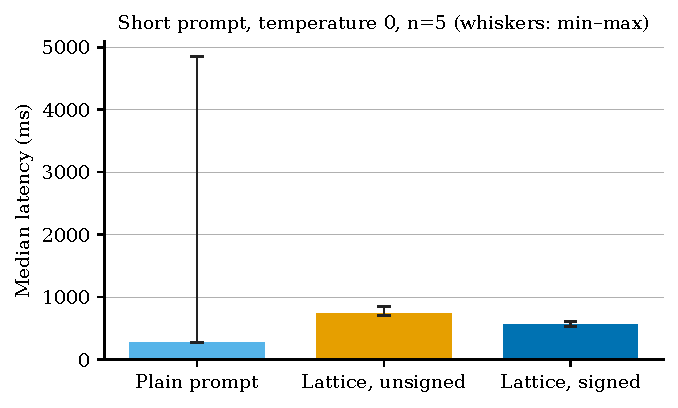
\includegraphics[width=\linewidth]{rw-latency.pdf}
\caption{Median latency of a one-line completion. Whiskers run from the minimum to the maximum of five trials. The plain arm sends only that line. The Lattice arms send the adapter's packed prompt.}
\label{fig:rw-latency}
\end{figure}

\begin{figure}[t]
\centering
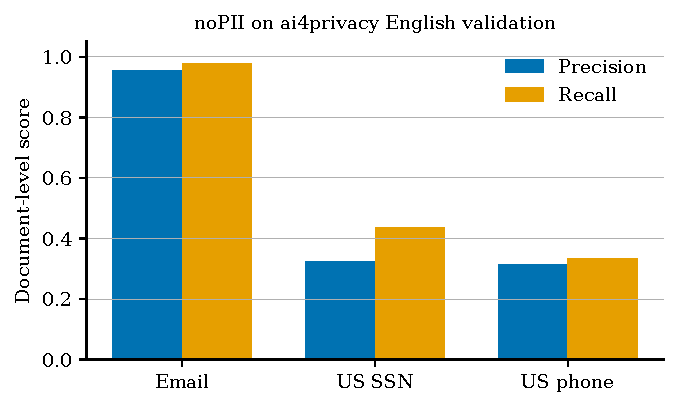
\includegraphics[width=\linewidth]{rw-pii.pdf}
\caption{Document-level precision and recall of the default \texttt{noPII} detectors at commit \texttt{ae99fb5} on ai4privacy English validation. US phone false positives still overlap social-security spans. US SSN false positives no longer overlap passport spans; recall is the remaining loss.}
\label{fig:rw-pii}
\end{figure}

\begin{figure}[t]
\centering
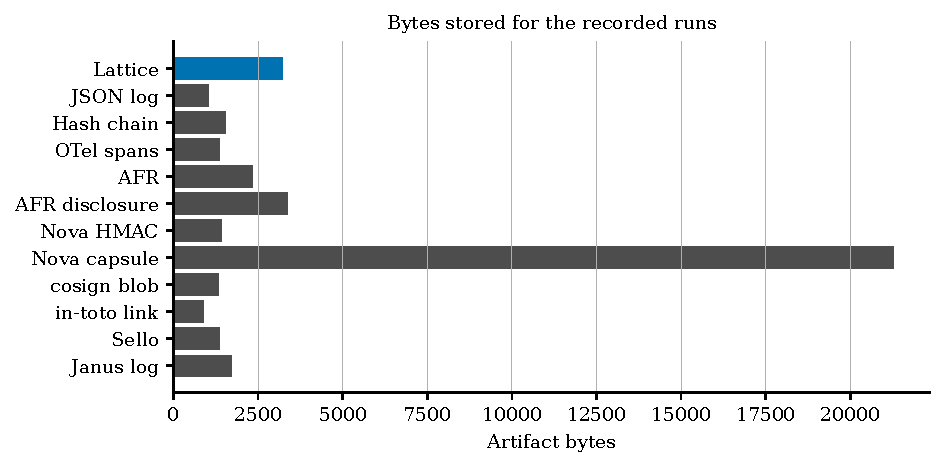
\includegraphics[width=0.92\linewidth]{rw-bytes.pdf}
\caption{Bytes retained for the recorded runs. Orange records keep the plaintext transcript; blue records keep only digests or ciphertext. The NovaFabric bar is one sealed capsule, not three hash receipts. AFR disclosure is the encrypted archive. The cosign bar is the blob, the signature, and the public key.}
\label{fig:rw-bytes}
\end{figure}

% Generated by eval/realworld/scripts/05-charts.py. Do not edit.
\begin{table*}[t]
\centering
\caption{Same recorded Ollama runs, wrapped by each system that ran. Wrap time excludes model generation. Wrap ms is one cold run per system, not a warmed median, and the scopes differ: Lattice and Sello are in-process JavaScript calls summed over three records, cosign and the NovaFabric capsule are one CLI invocation each, including process start and key loading, Janus reports whole milliseconds from its own timer, and the JSON log time is serialization only. PII in artifact reflects what the harness gave each system; where it is yes, the byte count includes the plaintext transcript. Signed output binding is yes when the record is signed and the system's own verifier rejected a byte edit. TrustTrack and Langfuse were not executed. The cosign run uploaded to the public Rekor log and verified online.}
\label{tab:rw-matrix}
\footnotesize
\resizebox{\textwidth}{!}{%
\begin{tabular}{@{}l l r r l l l l l@{}}
\toprule
System & Status & Wrap ms & Bytes & Offline verify & Byte edit detected & Key assumption & PII in artifact & Signed output binding \\
\midrule
Lattice receipt & measured & 5.923 & 3210 & yes & yes & other key rejected & no & yes \\
JSON log & baseline & 0.033 & 1045 & no & no & --- & yes & no \\
Hash chain & baseline & 0.082 & 1531 & yes & yes & rebuild accepted & yes & no \\
OTel GenAI spans & measured & 0.228 & 1366 & no & no & --- & yes & no \\
Agent Flight Recorder & measured & 0.797 & 2328 & yes & yes & mock anchor only & yes & no \\
AFR disclosure & measured & 1.907 & 3357 & yes & yes & mock anchor only & no & no \\
NovaFabric HMAC & measured & 0.077 & 1432 & yes & yes & shared secret re-signs & yes & no \\
NovaFabric capsule & measured & 1373.053 & 21288 & yes & yes & self-asserted key & yes & yes \\
cosign sign-blob & measured & 4916.329 & 1319 & online & yes & local key, Rekor upload & yes & yes \\
in-toto link & measured & 34.149 & 888 & yes & yes & functionary key & no & yes \\
Sello receipt & measured & 9.336 & 1359 & yes & yes & mock log & no & yes \\
Janus evidence log & measured & 5 & 1723 & yes & yes & writer key & yes & yes \\
TrustTrack & paper only & --- & --- & --- & --- & --- & --- & --- \\
Langfuse & not run & --- & --- & --- & --- & --- & --- & --- \\
\bottomrule
\end{tabular}}
\end{table*}


% Generated by eval/realworld/scripts/12-charts.py. Do not edit.
\providecommand{\citep}[1]{\cite{#1}}
\subsection{Broader comparison}
\label{sec:realworld-broad}
\emergencystretch=8em

This subsection adds the detector, citation, gateway, and hosted-model measurements from the same machine.

Lattice's OpenAI-compatible adapter called \path{https://openrouter.ai/api/v1}. The catalog check found 8 of the requested \texttt{:free} ids, and the listed prompt and completion prices were 0. Completed model rows: 8. Upstream HTTP 429 responses were retried. Pacing sleeps, that backoff, and the HTTP time of a failed attempt are excluded from Lattice time and from end-to-end time, so end-to-end time is Lattice processing plus the provider time of the attempt that returned. Provider time includes waiting for the response headers and reading the body. Completion tokens are capped at 8192. The adapter sends no temperature, \texttt{max\_tokens}, or reasoning field. A fetch wrapper adds temperature and the token cap to every request, and adds \texttt{reasoning.effort=low} for models whose catalog lists a reasoning parameter. A 400 that rejects that field is retried once without it. The Lattice rows therefore describe requests the adapter does not build on its own. Table~\ref{tab:rw-models} uses the provider string returned on the chat response. A drift cell is distinct successful answers, successful calls, and attempts. Output binding uses only calls that returned a receipt. The local row is the Ollama run in Section~\ref{sec:realworld} (drift n=3, overhead n=5). Hosted drift used n=10 when the call returned.
 On the local Ollama run, the median time outside the HTTP call was 2.4~ms (p95 15.0~ms, 0.439\% of that run's signed wall time). That localhost call returns the body with the headers, so the gap is processing time. Across hosted models with a successful signed short prompt, the median Lattice processing time was 1.10--1.69~ms, or 0.032--0.218\% of end-to-end time. Table~\ref{tab:rw-lattice} gives the median and p95 in milliseconds and as a percentage. The percentages are recomputed from the per-trial phase times; the \texttt{signedLatticePct} field stored in \texttt{openrouter.json} also counts the HTTP time of retried attempts. Lattice time includes \texttt{createAI()} construction and the fetch wrapper's JSON handling, so it is an upper bound. The packed Lattice prompt added 61--83 prompt tokens at the median versus the one-line direct prompt. The paired provider-time difference on that longer prompt had medians from -2398 to 3352~ms. A negative value means the packed call returned sooner. The difference changes sign and is often larger than a short extra prefill can explain, because completion length, including reasoning tokens, moves the provider time by seconds. It is reported separately and is not added to Lattice processing time.

\begin{table*}[t]
\centering
\caption{Short-prompt latency and the RAG, output-binding, ticket, and crew checks. Signed ms is the median of Lattice processing plus the provider time of the attempt that returned. Lattice ms is the median signed processing time, excluding provider time, retries, and backoff. Drift cells are unique successes / successes / attempts. Output binding counts receipts that verified and whose signed output hash matched the kept answer and changed after a one-character edit, among calls that returned a receipt. Receipt columns are the single-agent return and the crew return.}
\label{tab:rw-models}
\footnotesize
\resizebox{\textwidth}{!}{%
\begin{tabular}{@{}l l r r r r r l r l r r@{}}
\toprule
Model & Provider & Plain ms & Signed ms & Lattice ms & Drift 0 & Drift 0.7 & Cited & Output binding & Ticket leak & Agent rcpt & Crew rcpt \\
\midrule
llama3.2:3b local & Ollama & 278 & 559 & 2.45 & 1/3/3 & 1/3/3 & 3/3, 3/3 & 6/6 & no & 0 & 4 \\
\texttt{minimax/minimax-m3.1-flash:free} & Minimax & 3677 & 1489 & 1.69 & 3/10/10 & 1/10/10 & 10/10, 10/10 & 20/20 & no & 0 & 4 \\
\texttt{xingchen-agi/xing4.0-29b-a4b:free} & Phala & 3124 & 4812 & 1.21 & 4/8/10 & 3/3/10 & 8/8, 3/3 & 11/11 & no & 0 & 3 \\
\texttt{nvidia/nemotron-3.5-super-vl:free} & Nvidia & 675 & 845 & 1.20 & 1/10/10 & 2/10/10 & 10/10, 10/10 & 20/20 & no & 0 & 4 \\
\texttt{nvidia/nemotron-3.5-lightning:free} & Nvidia & 1319 & 2701 & 1.10 & 4/10/10 & 6/10/10 & 10/10, 10/10 & 20/20 & no & 0 & 3 \\
\texttt{dots-studio/dots-3-note-preview:free} & AtlasCloud & 1145 & 1275 & 1.50 & 2/10/10 & 3/10/10 & 10/10, 10/10 & 20/20 & no & 0 & 4 \\
\texttt{liquid/lfm-2.5-2.6b:free} & Liquid & 4179 & 4649 & 1.65 & 3/10/10 & 2/10/10 & 10/10, 10/10 & 20/20 & no & fail & fail \\
\texttt{thinkingmachines/inkling-small:free} & --- & --- & --- & --- & --- & --- & ---, --- & --- & --- & --- & --- \\
\texttt{poolside/laguna-s-2.1:free} & Poolside & 715 & 1413 & 1.56 & 1/10/10 & 4/10/10 & 10/10, 10/10 & 20/20 & no & 0 & 4 \\
\bottomrule
\end{tabular}}
\end{table*}

\begin{table*}[t]
\centering
\caption{Pure Lattice processing on the signed short prompt. The percentage is Lattice ms over Lattice ms plus the provider time of the attempt that returned; retried attempts, backoff, and pacing are excluded. Extra tokens are Lattice prompt tokens minus the direct prompt tokens. Provider delta is the signed provider time minus the direct provider time, in milliseconds, and is the latency of the longer packed prompt.}
\label{tab:rw-lattice}
\footnotesize
\resizebox{\textwidth}{!}{%
\begin{tabular}{@{}l r r r r r r@{}}
\toprule
Model & ms p50 & ms p95 & \% p50 & \% p95 & Extra tokens & Provider delta \\
\midrule
llama3.2:3b local & 2.45 & 14.96 & 0.439 & 2.469 & --- & --- \\
\texttt{minimax/minimax-m3.1-flash:free} & 1.69 & 3.66 & 0.218 & 0.327 & 63 & -2398 \\
\texttt{xingchen-agi/xing4.0-29b-a4b:free} & 1.21 & 3.50 & 0.032 & 0.033 & 83 & 3352 \\
\texttt{nvidia/nemotron-3.5-super-vl:free} & 1.20 & 2.03 & 0.138 & 0.260 & 80 & 169 \\
\texttt{nvidia/nemotron-3.5-lightning:free} & 1.10 & 1.96 & 0.053 & 0.082 & 82 & 1703 \\
\texttt{dots-studio/dots-3-note-preview:free} & 1.50 & 1.90 & 0.123 & 0.141 & 74 & 59 \\
\texttt{liquid/lfm-2.5-2.6b:free} & 1.65 & 4.09 & 0.035 & 0.076 & 61 & 1005 \\
\texttt{thinkingmachines/inkling-small:free} & --- & --- & --- & --- & --- & --- \\
\texttt{poolside/laguna-s-2.1:free} & 1.56 & 4.01 & 0.142 & 0.266 & 76 & 318 \\
\bottomrule
\end{tabular}}
\end{table*}

\path{thinkingmachines/inkling-small:free} is in the public catalog at price 0. Every measured call was rejected with HTTP 403 and the message that the model is only available on agentic harnesses, so this row has no latency sample.
\path{liquid/lfm-2.5-2.6b:free} returned HTTP 504 on the single-agent call (Provider returned error). That call is a provider failure, not a receipt or citation result.
\path{liquid/lfm-2.5-2.6b:free} returned HTTP 504 on the crew call (Provider returned error). That call is a provider failure, not a receipt or citation result.

On a 16$\times$16 solid red PNG, \path{nvidia/nemotron-3.5-super-vl:free} answered red from a direct \texttt{image\_url} part: yes (answer red). The Lattice image artifact answered red: no (answer blue). The PNG bytes were present in the Lattice request body: yes. The direct response provider was Nvidia. This vision call set \texttt{reasoning.effort=none}.
The text arms use reasoning.effort=low. On this vision call, effort low and effort minimal each spent 8192 completion tokens on reasoning and returned empty content. This recorded call sets reasoning.effort=none. Lattice inlines the PNG in the text JSON. The direct arm sends an image\_url part.
Lattice's OpenAI-compatible request builder, which the openai, xai, openrouter, and lm-studio adapters share, sends each artifact as a text part holding JSON and never emits an image part. A data-URL string is inlined as text and binary bytes are dropped, so the model received no image part, and the Lattice arm answered blue for a red PNG.

Document-level precision, recall, and F1 use the harness overlap rule: a document is a true positive when any predicted span of that type overlaps a gold span. An undefined F1 means there were no positive predictions, or no gold documents and no false positives. spaCy \texttt{en\_core\_web\_sm} emits none of the four labels, so its precision and F1 are undefined and its recall is zero wherever a gold span exists. Figure~\ref{fig:rw-pii-f1} omits those undefined bars.

The rule is not symmetric across tools. For each type, Lattice contributes every occurrence of the one substring \texttt{detect()} returns, while the other tools contribute every span they emit. When Lattice's one match falls on a different number, the document is a false positive and a false negative for Lattice, while a multi-span tool can still score it from another span. GLiNER \citep{gliner} is the general \path{urchade/gliner_small-v2.1} model, not a PII fine-tune, and its processor truncated each document to 384 tokens, while LLM Guard \citep{llmguard} scanned 1,500-character windows with 200 characters of overlap. LLM Guard ran its default Anonymize scanner with recognizer \path{Isotonic/deberta-v3-base_finetuned_ai4privacy_v2}, which was fine-tuned on ai4privacy, so its ai4privacy scores can be optimistic. A single process was OOM-killed on long inputs, so each batch of 250 documents ran in its own process with a fresh Vault. Raw SSN labels are mapped when the NER map returns them unchanged. Presidio \citep{presidio} used its pattern and spaCy \citep{spacy} recognizers for its four in-scope entities, with \texttt{en\_core\_web\_sm} rather than its default \texttt{en\_core\_web\_lg}. Lattice is an in-process JavaScript regex and the other detectors are Python pipelines, so Figure~\ref{fig:rw-pii-latency} compares runtimes as well as detectors. The Lattice rows were measured with the detectors at commit \texttt{a8cc091}; Section~\ref{sec:realworld} describes how the released detectors differ.

\begin{table*}[t]
\centering
\caption{ai4privacy English validation \citep{ai4privacy}, document level. Latency is the median milliseconds per document. Lattice rows use the detectors at commit \texttt{a8cc091}.}
\label{tab:rw-pii-ai4}
\footnotesize
\resizebox{\textwidth}{!}{%
\begin{tabular}{@{}l rrr rrr rrr rrr r@{}}
\toprule
Tool & \multicolumn{3}{c}{Email} & \multicolumn{3}{c}{US SSN} & \multicolumn{3}{c}{US phone} & \multicolumn{3}{c}{Card} & ms \\
& P & R & F1 & P & R & F1 & P & R & F1 & P & R & F1 & \\
\midrule
Lattice & 0.955 & 0.979 & 0.967 & 0.325 & 0.436 & 0.372 & 0.316 & 0.333 & 0.324 & 0.000 & --- & --- & 0.007 \\
presidio & 0.974 & 0.999 & 0.986 & 0.334 & 0.502 & 0.401 & 0.295 & 0.504 & 0.372 & 0.000 & --- & --- & 9.413 \\
spaCy sm & --- & 0.000 & --- & --- & 0.000 & --- & --- & 0.000 & --- & --- & --- & --- & 8.199 \\
gliner-small & 0.695 & 0.625 & 0.658 & 0.283 & 0.458 & 0.350 & 0.228 & 0.161 & 0.189 & 0.000 & --- & --- & 52.862 \\
llm-guard-anonymize & 0.965 & 0.999 & 0.982 & 0.991 & 0.450 & 0.619 & 0.650 & 0.962 & 0.776 & 0.000 & --- & --- & 142.115 \\
\bottomrule
\end{tabular}}
\end{table*}

\begin{table*}[t]
\centering
\caption{Gretel English finance test \citep{gretelfinance}, same document-level rule. Gold credit-card spans in this file use the label \texttt{credit\_card\_number}. Lattice rows use the detectors at commit \texttt{a8cc091}.}
\label{tab:rw-pii-gretel}
\footnotesize
\resizebox{\textwidth}{!}{%
\begin{tabular}{@{}l rrr rrr rrr rrr r@{}}
\toprule
Tool & \multicolumn{3}{c}{Email} & \multicolumn{3}{c}{US SSN} & \multicolumn{3}{c}{US phone} & \multicolumn{3}{c}{Card} & ms \\
& P & R & F1 & P & R & F1 & P & R & F1 & P & R & F1 & \\
\midrule
Lattice & 0.522 & 0.934 & 0.670 & 0.161 & 0.771 & 0.266 & 0.521 & 0.702 & 0.598 & 0.881 & 0.500 & 0.638 & 0.020 \\
presidio & 0.526 & 0.934 & 0.673 & 0.244 & 0.729 & 0.366 & 0.458 & 0.786 & 0.579 & 0.833 & 0.405 & 0.545 & 25.627 \\
spaCy sm & --- & 0.000 & --- & --- & 0.000 & --- & --- & 0.000 & --- & --- & 0.000 & --- & 21.623 \\
gliner-small & 0.237 & 0.511 & 0.324 & 0.090 & 0.557 & 0.155 & 0.338 & 0.234 & 0.277 & 0.165 & 0.500 & 0.248 & 156.490 \\
llm-guard-anonymize & 0.528 & 0.952 & 0.679 & 0.984 & 0.857 & 0.916 & 0.757 & 0.952 & 0.843 & 0.361 & 0.581 & 0.446 & 426.513 \\
\bottomrule
\end{tabular}}
\end{table*}

guardrails-detect-pii is from docs, not measured: ImportError: cannot import name 'DetectPII' from 'guardrails.hub'
nemo-guardrails is from docs, not measured: nemoguardrails is not installed, and en\_core\_web\_lg is not downloaded. The built-in sensitive-data rails call Presidio, which is scored on its own. The library also documents a separate GLiNER rail.

\begin{figure}[t]
\centering
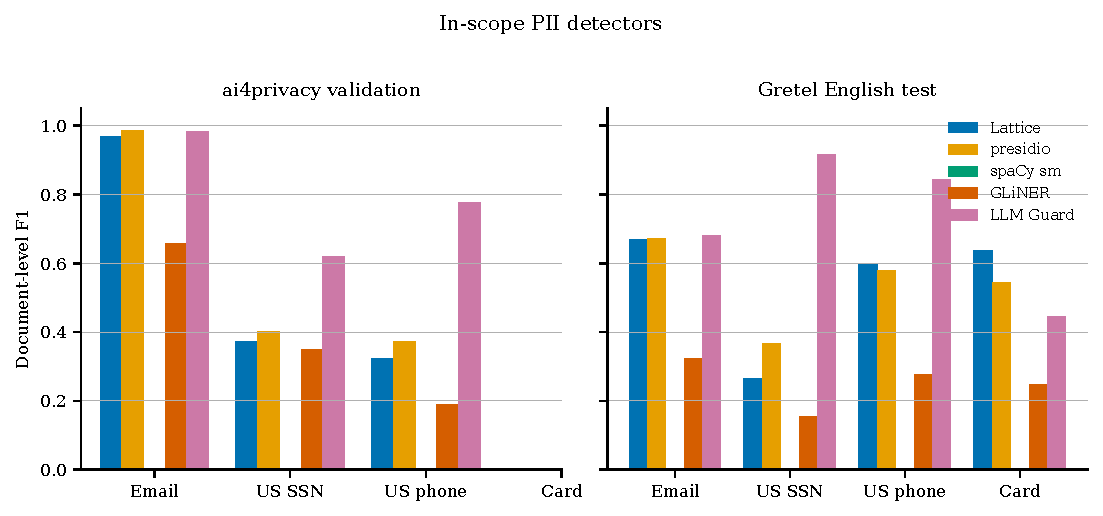
\includegraphics[width=\linewidth]{rw-pii-f1.pdf}
\caption{Document-level F1. A missing bar is an undefined F1.}
\label{fig:rw-pii-f1}
\end{figure}

\begin{figure}[t]
\centering
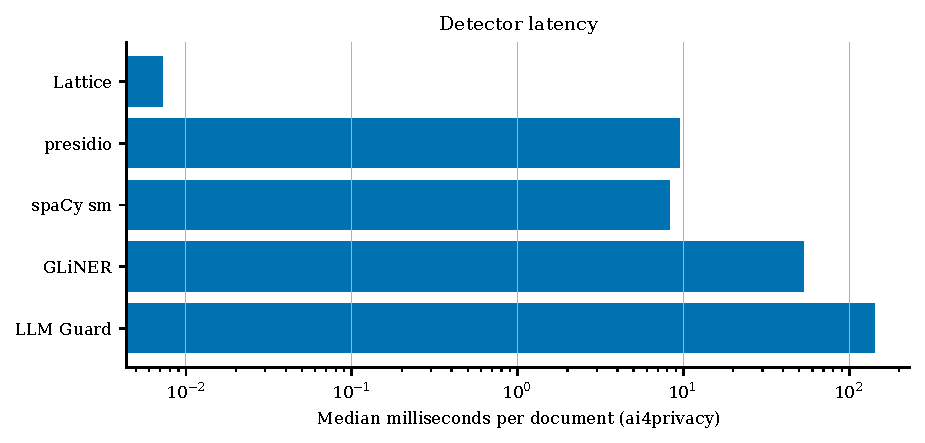
\includegraphics[width=0.86\linewidth]{rw-pii-latency.pdf}
\caption{Median detector time per ai4privacy document. The axis is logarithmic. Lattice runs in-process in JavaScript; the other detectors are Python pipelines.}
\label{fig:rw-pii-latency}
\end{figure}

On ASQA dev \citep{asqa} (n=948), a case-sensitive Wikipedia title substring matches 525 long answers and a case-insensitive substring matches 605. Square-bracket citations appear in 2 answers and overlap a gold title in 0. \texttt{mustCite} accepts a gold title in 7. These three checks are different predicates.
 A local cross-encoder, \path{typeform/distilbert-base-uncased-mnli}, scored 696 of 948 pairs and labeled 296 entailed (empty 252, NEUTRAL 211, CONTRADICTION 189, ENTAILMENT 296). Median classification time was 820.0~ms. The premise is the gold knowledge text truncated to 1,800 characters and the hypothesis is the long answer. Pairs with an empty premise or answer were not scored. This is a support label, not a citation-string check.

\begin{figure}[t]
\centering
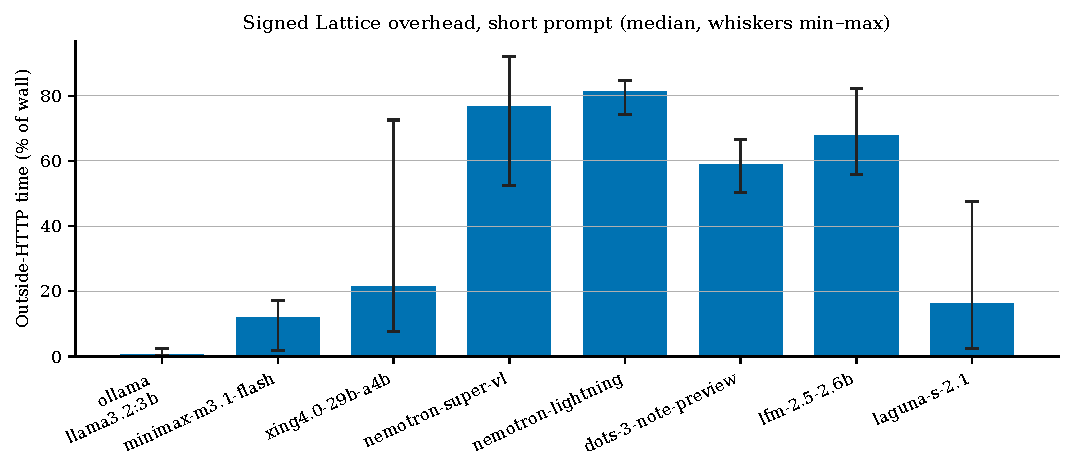
\includegraphics[width=\linewidth]{rw-overhead-pct.pdf}
\caption{Signed Lattice processing time as a percentage of end-to-end time, where end-to-end time is Lattice processing plus the provider time of the attempt that returned. Retried attempts, backoff, and pacing are excluded. The bar is the median and the whiskers run from the minimum to the maximum. The local bar is wall time minus the localhost HTTP call in the Ollama run of Section~\ref{sec:realworld}.}
\label{fig:rw-overhead-pct}
\end{figure}

\begin{figure}[t]
\centering
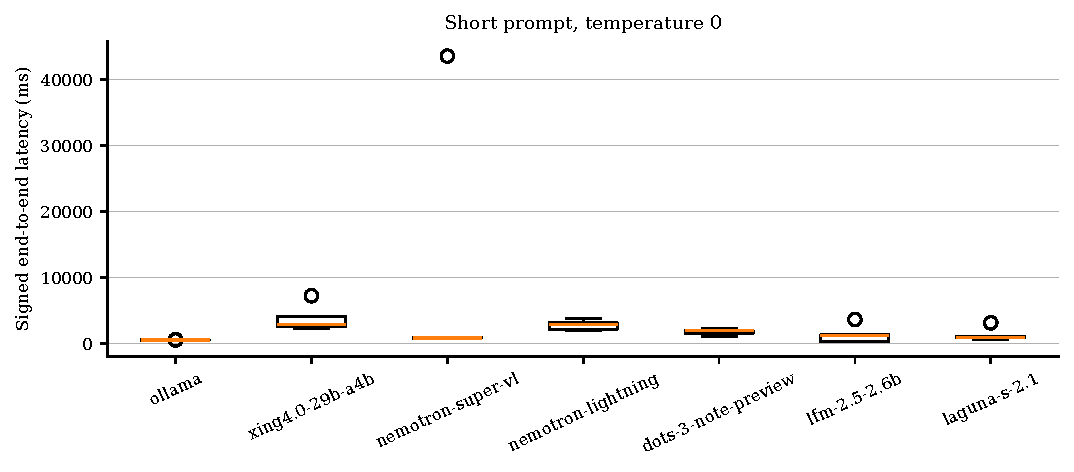
\includegraphics[width=\linewidth]{rw-latency-dist.pdf}
\caption{Signed short-prompt latency. Ollama is five trials. Each hosted row is the successful signed trials, as Lattice processing plus the provider time of the attempt that returned.}
\label{fig:rw-latency-dist}
\end{figure}

\begin{figure}[t]
\centering
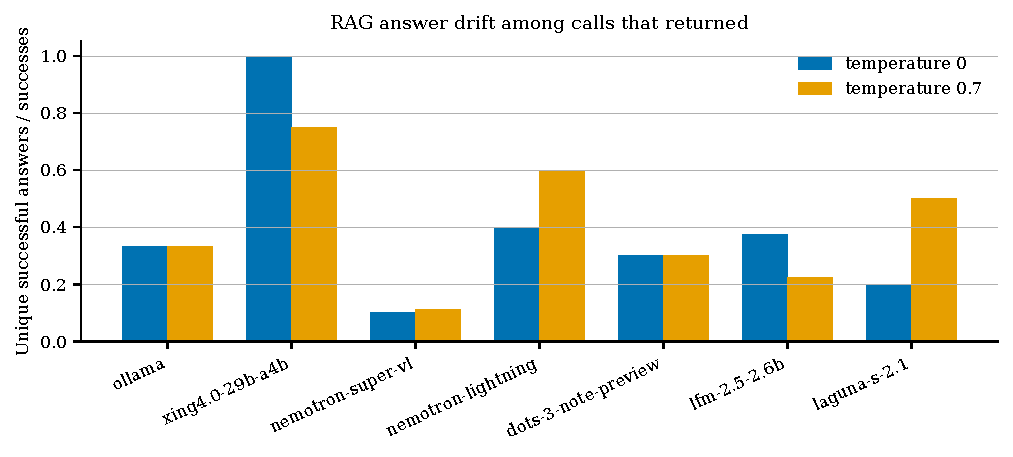
\includegraphics[width=\linewidth]{rw-drift.pdf}
\caption{Distinct successful RAG answers divided by the number of successful calls. Ollama used n=3. Hosted rows use the successes recorded for that model.}
\label{fig:rw-drift}
\end{figure}

\begin{figure}[t]
\centering
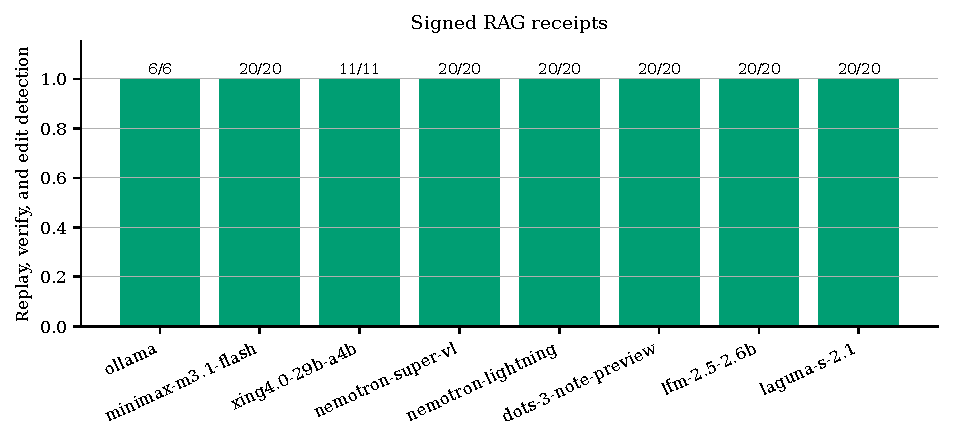
\includegraphics[width=0.9\linewidth]{rw-replay.pdf}
\caption{Signed output binding on receipts from calls that returned. A receipt counts when it verified, its signed output hash matched the kept answer, and a one-character edit of that answer changed the hash. \texttt{replayOffline} returns the outputs the caller supplies, so this is a hash-binding check, not a re-run of the model. Rate-limited calls with no receipt are left out of the denominator.}
\label{fig:rw-replay}
\end{figure}

\begin{figure}[t]
\centering
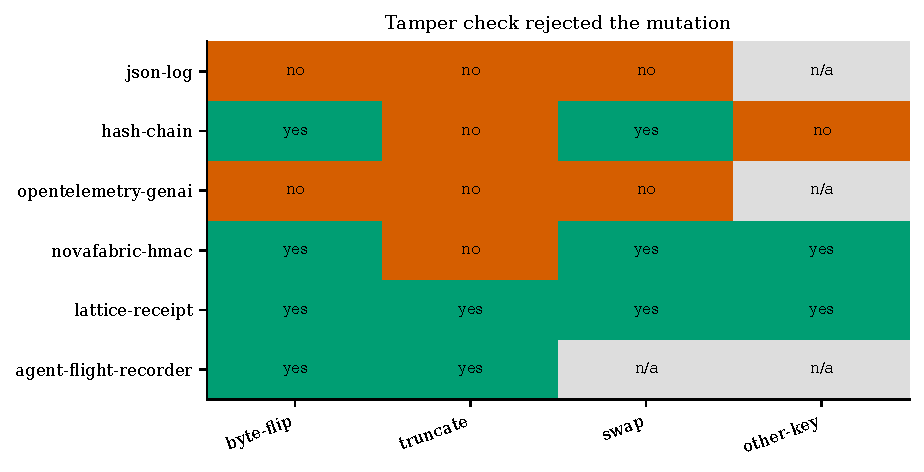
\includegraphics[width=\linewidth]{rw-tamper-heat.pdf}
\caption{Whether the system's own check rejects the mutation. Gray means that class was not applied. Truncating a hash chain leaves a valid prefix. A byte flip inside a JSON string, a dropped tail record, and a swapped response all remain valid JSON, so a parser does not catch them.}
\label{fig:rw-tamper-heat}
\end{figure}

\begin{figure}[t]
\centering
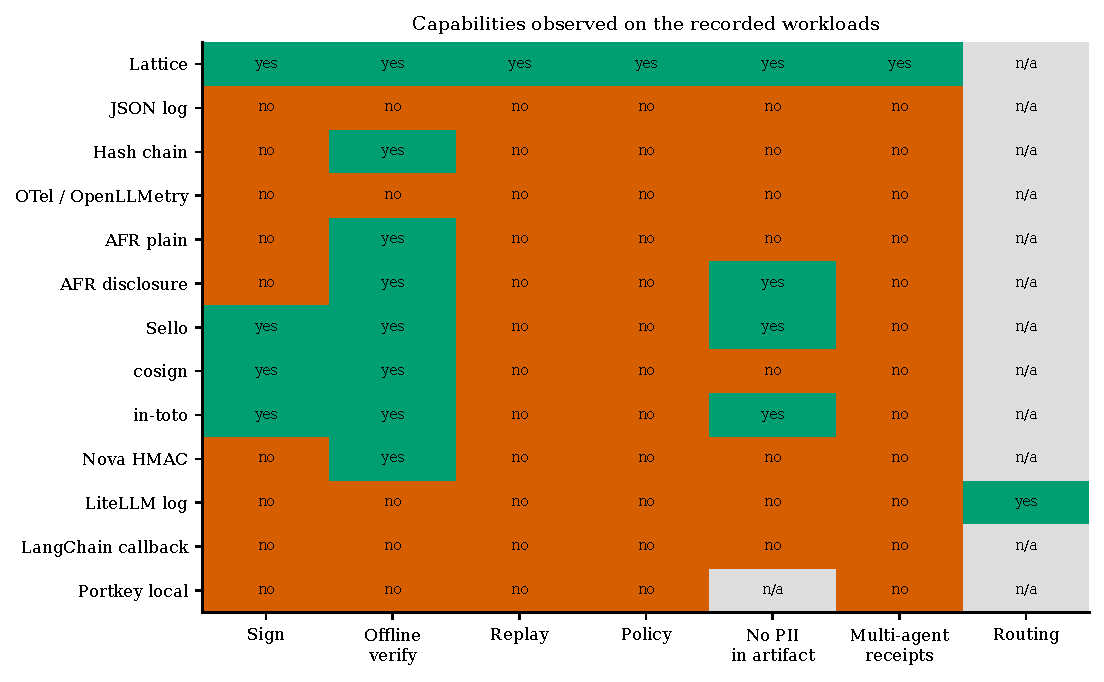
\includegraphics[width=\linewidth]{rw-capability.pdf}
\caption{Capabilities observed on these workloads. Gray is not measured here. Signed output binding is yes when the system signs the record and its own verifier rejected a byte edit of the stored record; for Lattice the signed output hash is checked by re-hashing the kept answer. cosign's offline-verify cell is gray because the measured \texttt{verify-blob} checked the Rekor log online. LiteLLM routing is eight calls across two identical local deployments, which returned one route. Lattice routing is gray because each live call used one configured provider. Portkey's stored-log endpoint returned HTTP 500, so the PII cell is gray. LiteLLM's callback log stored the prompt text. The single-agent Lattice return carried no receipt; the crew return did.}
\label{fig:rw-capability}
\end{figure}

LiteLLM \citep{litellm} here is an in-process client, not a proxy process. Its router sent eight short prompts to two identical Ollama deployments and returned 1 distinct route across 8 calls. That is a weak determinism check. The other wrappers are a LangChain callback handler \citep{langchain}, OpenLLMetry's in-process spans \citep{openllmetry}, and a local Portkey gateway \citep{portkey}. Helicone and Langfuse were not started.
 The latency rows are small samples (n=3--5 per arm). Each wrapper ran its calls in its own block, not interleaved with the direct arm, against \texttt{llama3.2:3b} on a CPU-only host. The min--max ranges overlap, so the p50 order reflects generation noise, not wrapper overhead.

\begin{table*}[t]
\centering
\caption{Local wrappers around Ollama. Marker detection scans the captured log or span. Portkey's log route failed, so that row does not show what a stored log would contain. None of these logs is signed.}
\label{tab:rw-gateways}
\footnotesize
\resizebox{\textwidth}{!}{%
\begin{tabular}{@{}l l r r r r l l l@{}}
\toprule
System & Status & n & p50 ms & min--max ms & Bytes & Markers in capture & Offline verify & Signed output binding \\
\midrule
ollama-direct & measured & 5 & 1060.2 & 435--1833 & --- & --- & --- & --- \\
litellm & measured & 5 & 3964.8 & 587--6363 & 2408 & prompt stored & no & no \\
langchain-callback & measured & 5 & 1936.3 & 844--8321 & 6893 & yes & no & no \\
openllmetry & measured & 3 & 1253.1 & 1211--1329 & 3346 & yes & no & no \\
portkey-gateway & measured & 5 & 6281.0 & 1099--8688 & 1953 & log unread & no & no \\
helicone & from docs, not measured & --- & --- & --- & --- & --- & --- & --- \\
langfuse & from docs, not measured & --- & --- & --- & --- & --- & --- & --- \\
\bottomrule
\end{tabular}}
\end{table*}

\begin{figure}[t]
\centering
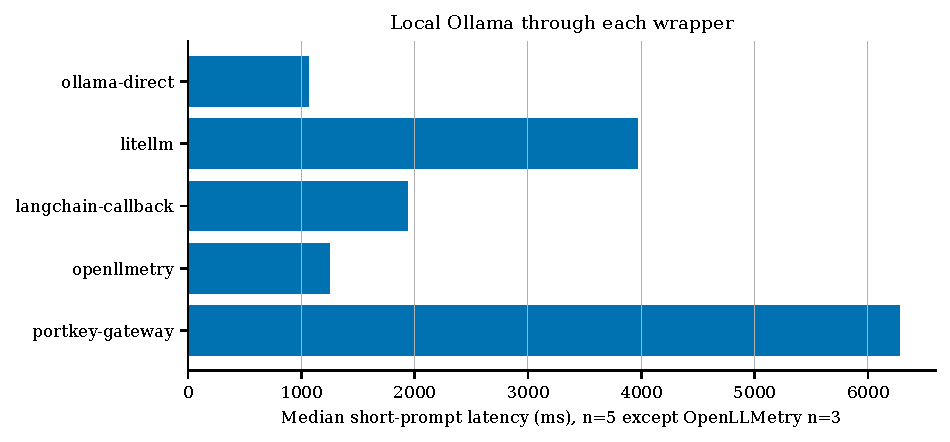
\includegraphics[width=0.86\linewidth]{rw-gateway-latency.pdf}
\caption{Short-prompt latency through each local wrapper: median, with whiskers from the minimum to the maximum. OpenLLMetry used n=3. The other measured rows used n=5. The arms ran one after another on a CPU-only host, so the order is not a ranking of wrapper overhead.}
\label{fig:rw-gateway-latency}
\end{figure}



\section{Discussion}

Signed capability receipts change what is possible after a run. An operator can hand a
receipt and the kept output to an auditor who verifies the receipt with a public key and
checks the output against it offline, without access to the original system. The check
shows that the output is the one the key holder signed, not that the key holder reported
the run honestly. A dispute about what a
system produced becomes a check against a signed artifact rather than an argument about
log files. A continuous integration pipeline can use the \code{eval} subcommand to gate
regressions in cost, in determinism, and in quality across a corpus of receipts, which
makes a model or prompt change a reviewable event with measurable consequences. The
package itself is published with provenance, so an operator can check that the runtime
it deploys was built from the published source. A receipt does not record which build
of the runtime produced it.

The design has also been tested from outside. An independent evaluation harness run
against release 1.5.1 \cite{latticeissue21} found three gaps: a violated
no-personally-identifiable-information invariant copied the matched substring into the
signed evidence while the redaction manifest claimed it had been redacted; receipts
carried no freshness or audience binding, so a valid receipt could be replayed to a
different relying party at any later time; and crew receipts formed a tree that no
verifier checked as a whole. Release 1.6.0 \cite{latticepr22} added evidence redaction,
the audience, nonce, and expiry fields, and \code{verifyChain}. Matched personal data is
rewritten to a detector name, a length, and a mask before signing. An issuer's
\code{expiresAt} is always enforced, while audience, nonce, maximum age, and the
schema-version floor remain verifier opt-ins, so an older receipt still verifies.
\code{verifyChain} checks every link, the single root, and parent reachability, and its
failures are a \code{VerifyChainErrorKind}, not one of the ten \code{VerifyErrorKind}
values. An open chain fails on tail truncation only when the caller passes an expected
count; otherwise the result carries a \code{tail-truncation-unchecked} warning. A crew
run closes its chain with a receipt that lists every other member, so a dropped leaf
fails verification without that count, and verifiers in the 1.6.x releases do not
enforce that closure (Section~\ref{sec:chains}). \code{lattice verify} and
\code{lattice receipt verify-chain} print \code{WARN} lines for commitments that were
not checked, such as an audience the caller did not pass or an open chain verified
without a count, and, unless \code{--quiet} is set, \code{INFO} lines for optional checks
the receipt does not use. The commit and hardware of each harness run are recorded in
Appendix~\ref{app:repro} and in \code{eval/results/}.

Three design tensions are worth naming. The first is determinism against model
nondeterminism. Models are not deterministic, so Lattice does not promise to reproduce a
live call. It promises to bind the input-artifact hashes and a kept output to a signed
record, and it offers a layered determinism check in the evaluation tool for free
form text. The second is redaction against reproducibility. A receipt that redacts a
secret cannot reproduce a run that depended on that secret value, so redaction is scoped
to material that must never be shared, and the redaction manifest makes the omission
explicit and signed. The third is modularity against uniformity. Provider-only
consumers can opt into native tools and structured outputs, while the default runtime
and agent paths preserve their existing portable behavior. We accept this explicit
split because parity is what makes a receipt portable.

% --- Limitations ----------------------------------------------------------
\section{Limitations}

Several limitations follow directly from the design. Replay checks a kept output against
the signed output hash and does not call a model, so a receipt is evidence about a past
run rather than a way to obtain new model behavior. Semantic determinism for free-form
text relies on a layered judge in the evaluation tool, which is more expensive and less
crisp than an exact hash match. The capability registry is a point-in-time snapshot
refreshed by continuous integration, so a brand new model may be absent until the next
refresh, although capability negotiation can refine a profile at call time.

A receipt signs less than a full record of the run. It commits to input-artifact
hashes, the output hash, the contract hash, and the selected route, but not to the task
text, the packed prompt, the policy, or the routing candidates and reasons, so two runs
with different instructions but the same artifacts, output, and token usage produce
receipts that differ only in identifiers and times. Receipts are signed by the issuing
runtime, so they show integrity and the signing key, not that the issuer reported the
run honestly. The hashes are unsalted, so a low-entropy input or output can be
confirmed from a receipt by guessing. Single-agent runs return no receipt:
\code{ai.runAgent} sends its checkpoint receipts to a tracer only, and only
\code{ai.run} and crews return receipts to the caller. The five OpenAI-shaped adapters
send artifacts as JSON text, drop values that are not strings, such as binary image
bytes and JSON objects, and still hash the dropped input,
so for those adapters an input hash does not show that the model received the input;
in the hosted vision probe the Lattice arm answered blue for a red image while a direct
image part answered red (Section~\ref{sec:realworld-broad}). When a configured signer
fails, the runtime does not hide the gap: by default the result carries a receipt error
field and an event, and an operator can instead configure the run to fail.

The default personally identifiable information detectors are regular expressions over
four United States and email formats documented in the source. Names, addresses, and
non-United States formats are not detected. Identifier labels and type cues trade recall
against precision: a real number right after a label such as \code{ref}, or a bare
number without its cue, is missed, and long Luhn-valid identifiers are flagged. On
public data the social security and phone detectors confuse identifiers of the same
shape, such as passport numbers, and score far below the synthetic harness
(Table~\ref{tab:rw-pii-ai4}). Those public-data rows were measured with the detectors
at commit \code{a8cc091}, which differ from the rules above as
Section~\ref{sec:realworld} describes. The must-cite invariant is syntactic. By default it reads
only citation lists, and its prose options check markers, not whether the cited
artifact supports the claim. Long-form ASQA answers carry no citation list, so the
default accepts a gold title in none of them; the count in Section~\ref{sec:realworld}
was measured at commit \code{a8cc091}, where an inline marker containing the name
counted by default.

No replay cache ships with the verifier, so a relying party that must accept a receipt
only once keeps its own record of accepted content identifiers. An open chain warns on
tail truncation unless an expected count is passed. A crew's closing receipt makes a
dropped leaf a count mismatch without an out-of-band count, but a verifier from the
1.6.x releases does not enforce it, and a missing closer leaves the closed chain
unverifiable. Finally, external audit helpers can sign and replay evidence produced
elsewhere, but they cannot prove that the external executor used the claimed provider
unless that executor supplies trustworthy raw envelopes. The hosted measurements use
free endpoints. They rate-limit, they are not a paid-latency sample, and a model that
rejects ordinary chat calls is reported as unavailable rather than given a latency.
Paired provider times are too noisy to treat as the cost of the extra prompt tokens
Lattice packs.

% --- Future Work ----------------------------------------------------------
\section{Future Work}

Several extensions build naturally on the receipt primitive. Receipts can commit to a
hash of the task, the packed prompt, and the policy, and can use salted or keyed
commitments for low-entropy values. The OpenAI-shaped adapters can send native image
parts, or fail a run whose artifact they cannot package, so that an input hash always
names an input the provider received. \code{ai.runAgent} can return its checkpoint
receipts and a closing receipt to the caller. External audit can become
stronger when executors attach provider-side attestations or gateway signed envelopes.
The run event vocabulary can be exported more broadly through OpenTelemetry
\cite{opentelemetry} so receipts and traces share a vocabulary across organizations.
Key management can be hardened with key management service backed signers and rotation
policies. Realtime audio and video sessions need a distinct session surface and a
session summary receipt, since a bidirectional stream differs structurally from a
request and response. Finally, the modular subpaths can be validated against more
downstream runtimes so adoption does not require replacing an existing orchestration
stack.

% --- Conclusion -----------------------------------------------------------
\section{Conclusion}

Production systems built on large language models need runs that an auditor can verify
and an operator can reproduce. We presented Lattice, a capability-first runtime in which
a signed model run emits a capability receipt that is canonicalized, redacted before
signing, and signed inside a Dead Simple Signing Envelope, backed by a deterministic and
inspectable router and by output invariants with terminal semantics. The receipt binds
the input-artifact hashes, the output hash, the contract hash, and the selected route; it
does not record the task text, the policy, or why the route was chosen. A verifier can
check a receipt with a public key and confirm offline that a kept output hashes to the
signed value. The implementation ships publicly with supply-chain provenance, a
seven-provider parity contract over one receipt format, a registry of 332 model profiles,
modular adoption paths, a measured signing and verification cost
(Table~\ref{tab:bench}), and a test suite that encodes the guarantees as invariants. By
making a signed receipt a byproduct of every \code{ai.run} call and crew run that has a
signer, Lattice turns auditability from after-the-fact instrumentation into a property of the
runtime itself.

% --- Reproducibility ------------------------------------------------------
\section{Reproducibility notes}
\label{app:repro}

% bench-platform:begin
The benchmark in \code{paper/bench/results.json} was produced by \code{scripts/bench-receipts.mjs} on Node v24.22.1 (linux 6.12.94+ x64), processor Intel(R) Xeon(R) Processor, Lattice 1.6.0, commit \code{4549334}. Provider: mocked (createFakeProvider), no network.
% bench-platform:end

The packages \code{@full-self-browsing/lattice} and \code{@full-self-browsing/lattice-cli} are published on the public npm registry with an OpenID Connect trusted publisher and with supply-chain provenance attestations in the spirit of SLSA \cite{slsa}. A tagged GitHub release accompanies each publish. The runtime targets Node 24 or newer. Modular subpaths for audit, context, artifacts, routing, tools, eval, and core are also exercised as Node-20-style consumers in the test suite.

The command-line tool returns exit status 0 for success, 1 for a verification or test failure, and 2 for a load or configuration failure. A successful \code{verify} or \code{receipt verify-chain} prints advisory lines on standard error, each with an advisory code: \code{WARN} lines always and \code{INFO} lines unless \code{--quiet} is set. The process still exits 0, so a caller gates on the codes. \code{receipt verify-chain} also accepts \code{--require-closure} and \code{--partial}, and a malformed closing receipt fails with a typed \code{FAIL kind=} line.

The offline evaluation harness lives in \code{eval/}. \code{eval/run-all.sh} rebuilds the packages and writes \code{eval/results/}, including hardware and the git commit. Provider calls in that harness are in-process fakes. No API key is required.

% --- Acknowledgment -------------------------------------------------------
\section*{Acknowledgment}

The evaluation uses the ai4privacy pii-masking-300k dataset \cite{ai4privacy} under its
terms for academic, non-commercial use with acknowledgement, the Gretel synthetic PII
finance dataset \cite{gretelfinance}, and the ASQA dataset \cite{asqa}. The committed
results hold aggregate scores, not dataset records.
% TODO(authors): confirm that the ai4privacy non-commercial terms cover this use, given
% the first author's company affiliation.

% --- References -----------------------------------------------------------
\bibliographystyle{IEEEtran}
\bibliography{refs}

\end{document}
